\chapter{Bijou 7.2.0 Release Evidence}\label{record-261}

\noindent{\footnotesize\color{BookMuted}\path{docs/releases/7.2.0/README.md}\par}\smallskip

Bijou 7.2.0 is a narrow stabilization and demo-integrity release after the 7.1.0 release-video rehearsal exposed user-facing seams in framework input, DOGFOOD localization and themes, Blocks documentation, release-story surfaces, dependency posture, and release bookkeeping.

This packet was started on the release-gate branch, finalized on the release-prep branch, and closed from the verified \texttt{o\allowbreak{}r\allowbreak{}i\allowbreak{}g\allowbreak{}i\allowbreak{}n\allowbreak{}/\allowbreak{}m\allowbreak{}a\allowbreak{}i\allowbreak{}n} release commit. The public \texttt{v\allowbreak{}7\allowbreak{}.\allowbreak{}2\allowbreak{}.\allowbreak{}0} tag was created from \texttt{1\allowbreak{}2\allowbreak{}3\allowbreak{}f\allowbreak{}4\allowbreak{}a\allowbreak{}6\allowbreak{}1\allowbreak{}5\allowbreak{}0\allowbreak{}9\allowbreak{}6\allowbreak{}3\allowbreak{}9\allowbreak{}3\allowbreak{}2\allowbreak{}1\allowbreak{}1\allowbreak{}8\allowbreak{}c\allowbreak{}b\allowbreak{}f\allowbreak{}7\allowbreak{}6\allowbreak{}3\allowbreak{}a\allowbreak{}8\allowbreak{}a\allowbreak{}6\allowbreak{}e\allowbreak{}c\allowbreak{}0\allowbreak{}3\allowbreak{}4\allowbreak{}8\allowbreak{}7\allowbreak{}e\allowbreak{}2\allowbreak{}2\allowbreak{}7} on 2026-07-05 after final-main validation passed. Tag Guard, Release workflow, tag CI, GitHub Release verification, and npm registry verification all passed after the tag was pushed.

\section{Release Summary}\label{record-261-release-summary}

\begin{itemize}
\tightlist
\item
  Version: \texttt{7\allowbreak{}.\allowbreak{}2\allowbreak{}.\allowbreak{}0}
\item
  Tag: \href{https://github.com/flyingrobots/bijou/releases/tag/v7.2.0}{\texttt{v\allowbreak{}7\allowbreak{}.\allowbreak{}2\allowbreak{}.\allowbreak{}0}}
\item
  Previous public tag: \texttt{v\allowbreak{}7\allowbreak{}.\allowbreak{}1\allowbreak{}.\allowbreak{}0}
\item
  Release commit: \texttt{1\allowbreak{}2\allowbreak{}3\allowbreak{}f\allowbreak{}4\allowbreak{}a\allowbreak{}6\allowbreak{}1\allowbreak{}5\allowbreak{}0\allowbreak{}9\allowbreak{}6\allowbreak{}3\allowbreak{}9\allowbreak{}3\allowbreak{}2\allowbreak{}1\allowbreak{}1\allowbreak{}8\allowbreak{}c\allowbreak{}b\allowbreak{}f\allowbreak{}7\allowbreak{}6\allowbreak{}3\allowbreak{}a\allowbreak{}8\allowbreak{}a\allowbreak{}6\allowbreak{}e\allowbreak{}c\allowbreak{}0\allowbreak{}3\allowbreak{}4\allowbreak{}8\allowbreak{}7\allowbreak{}e\allowbreak{}2\allowbreak{}2\allowbreak{}7}
\item
  Release type: stable minor
\item
  npm dist-tag after publish: \texttt{l\allowbreak{}a\allowbreak{}t\allowbreak{}e\allowbreak{}s\allowbreak{}t}
\item
  Release-prep branch: \texttt{c\allowbreak{}y\allowbreak{}c\allowbreak{}l\allowbreak{}e\allowbreak{}/\allowbreak{}v\allowbreak{}7\allowbreak{}2\allowbreak{}-\allowbreak{}r\allowbreak{}e\allowbreak{}l\allowbreak{}e\allowbreak{}a\allowbreak{}s\allowbreak{}e\allowbreak{}-\allowbreak{}p\allowbreak{}r\allowbreak{}e\allowbreak{}p}
\item
  Release-gate lineage branch: \texttt{c\allowbreak{}y\allowbreak{}c\allowbreak{}l\allowbreak{}e\allowbreak{}/\allowbreak{}v\allowbreak{}7\allowbreak{}2\allowbreak{}-\allowbreak{}r\allowbreak{}e\allowbreak{}l\allowbreak{}e\allowbreak{}a\allowbreak{}s\allowbreak{}e\allowbreak{}-\allowbreak{}g\allowbreak{}a\allowbreak{}t\allowbreak{}e\allowbreak{}-\allowbreak{}3\allowbreak{}5\allowbreak{}4}
\item
  Release date: 2026-07-05
\item
  Publish surface: npm workspace packages only
\item
  Release workflow: \url{https://github.com/flyingrobots/bijou/actions/runs/28736930944}
\end{itemize}

\section{Tracker And Goalpost Map}\label{record-261-tracker-and-goalpost-map}

Each goalpost records the release-law evidence required by \href{https://github.com/flyingrobots/bijou/blob/cbd70612140e7a450d764b3c7be1c6af878b99bc/docs/release.md}{\texttt{d\allowbreak{}o\allowbreak{}c\allowbreak{}s\allowbreak{}/\allowbreak{}r\allowbreak{}e\allowbreak{}l\allowbreak{}e\allowbreak{}a\allowbreak{}s\allowbreak{}e\allowbreak{}.\allowbreak{}m\allowbreak{}d}}: tracker, design, PRs, completed slices, deterministic proof or fixture, replay command, witness, and residual-risk disposition.

\subsection{V7.2 Stabilization Goalpost}\label{record-261-v7.2-stabilization-goalpost}

\begin{itemize}
\tightlist
\item
  Tracker: \href{https://github.com/flyingrobots/bijou/issues/354}{\#354}.
\item
  Design lineage: \href{https://github.com/flyingrobots/bijou/blob/cbd70612140e7a450d764b3c7be1c6af878b99bc/docs/design/RE-041-v72-framework-input-stabilization.md}{\texttt{R\allowbreak{}E\allowbreak{}-\allowbreak{}0\allowbreak{}4\allowbreak{}1}}, \href{https://github.com/flyingrobots/bijou/blob/cbd70612140e7a450d764b3c7be1c6af878b99bc/docs/design/DX-047-blocks-app-binding-snippets.md}{\texttt{D\allowbreak{}X\allowbreak{}-\allowbreak{}0\allowbreak{}4\allowbreak{}7}}, \href{https://github.com/flyingrobots/bijou/blob/cbd70612140e7a450d764b3c7be1c6af878b99bc/docs/design/DL-017-dogfood-light-theme-readiness.md}{\texttt{D\allowbreak{}L\allowbreak{}-\allowbreak{}0\allowbreak{}1\allowbreak{}7}}, \href{https://github.com/flyingrobots/bijou/blob/cbd70612140e7a450d764b3c7be1c6af878b99bc/docs/design/DL-018-first-party-theme-variant-coverage.md}{\texttt{D\allowbreak{}L\allowbreak{}-\allowbreak{}0\allowbreak{}1\allowbreak{}8}}, \href{https://github.com/flyingrobots/bijou/blob/cbd70612140e7a450d764b3c7be1c6af878b99bc/docs/design/LX-020-dogfood-locale-demo-readiness.md}{\texttt{L\allowbreak{}X\allowbreak{}-\allowbreak{}0\allowbreak{}2\allowbreak{}0}}, and \href{https://github.com/flyingrobots/bijou/blob/cbd70612140e7a450d764b3c7be1c6af878b99bc/docs/design/DF-078-dogfood-release-story-surfaces.md}{\texttt{D\allowbreak{}F\allowbreak{}-\allowbreak{}0\allowbreak{}7\allowbreak{}8}}.
\item
  Landed PRs: \href{https://github.com/flyingrobots/bijou/pull/355}{\#355}, \href{https://github.com/flyingrobots/bijou/pull/359}{\#359}, \href{https://github.com/flyingrobots/bijou/pull/360}{\#360}, \href{https://github.com/flyingrobots/bijou/pull/361}{\#361}, \href{https://github.com/flyingrobots/bijou/pull/362}{\#362}, \href{https://github.com/flyingrobots/bijou/pull/453}{\#453}, \href{https://github.com/flyingrobots/bijou/pull/452}{\#452}, and \href{https://github.com/flyingrobots/bijou/pull/460}{\#460}.
\item
  Completed slices: framework input fallthrough and helper exports, DOGFOOD locale fallback honesty, DOGFOOD light-theme readability, first-party theme variant coverage, Blocks app-binding snippets, mouse hover tracking, and in-app release-story surfaces.
\item
  Canonical proof inputs: the tests and DOGFOOD fixtures named in the per-slice sections below.
\item
  Replay: run \texttt{n\allowbreak{}p\allowbreak{}m\allowbreak{} \allowbreak{}r\allowbreak{}u\allowbreak{}n\allowbreak{} \allowbreak{}r\allowbreak{}e\allowbreak{}l\allowbreak{}e\allowbreak{}a\allowbreak{}s\allowbreak{}e\allowbreak{}:\allowbreak{}r\allowbreak{}e\allowbreak{}a\allowbreak{}d\allowbreak{}i\allowbreak{}n\allowbreak{}e\allowbreak{}s\allowbreak{}s} from the release-prep branch, then run \texttt{n\allowbreak{}p\allowbreak{}m\allowbreak{} \allowbreak{}r\allowbreak{}u\allowbreak{}n\allowbreak{} \allowbreak{}r\allowbreak{}e\allowbreak{}l\allowbreak{}e\allowbreak{}a\allowbreak{}s\allowbreak{}e\allowbreak{}:\allowbreak{}r\allowbreak{}e\allowbreak{}a\allowbreak{}d\allowbreak{}i\allowbreak{}n\allowbreak{}e\allowbreak{}s\allowbreak{}s\allowbreak{} \allowbreak{}-\allowbreak{}-\allowbreak{} \allowbreak{}-\allowbreak{}-\allowbreak{}m\allowbreak{}i\allowbreak{}l\allowbreak{}e\allowbreak{}s\allowbreak{}t\allowbreak{}o\allowbreak{}n\allowbreak{}e\allowbreak{} \allowbreak{}v\allowbreak{}7\allowbreak{}.\allowbreak{}2\allowbreak{}.\allowbreak{}0} again from the exact merged final-main release commit before tagging.
\item
  Witness: local release-gate validation on 2026-07-04 passed \texttt{n\allowbreak{}p\allowbreak{}m\allowbreak{} \allowbreak{}r\allowbreak{}u\allowbreak{}n\allowbreak{} \allowbreak{}r\allowbreak{}e\allowbreak{}l\allowbreak{}e\allowbreak{}a\allowbreak{}s\allowbreak{}e\allowbreak{}:\allowbreak{}p\allowbreak{}r\allowbreak{}e\allowbreak{}f\allowbreak{}l\allowbreak{}i\allowbreak{}g\allowbreak{}h\allowbreak{}t}, \texttt{n\allowbreak{}p\allowbreak{}m\allowbreak{} \allowbreak{}r\allowbreak{}u\allowbreak{}n\allowbreak{} \allowbreak{}d\allowbreak{}o\allowbreak{}c\allowbreak{}s\allowbreak{}:\allowbreak{}i\allowbreak{}n\allowbreak{}v\allowbreak{}e\allowbreak{}n\allowbreak{}t\allowbreak{}o\allowbreak{}r\allowbreak{}y}, \texttt{n\allowbreak{}p\allowbreak{}m\allowbreak{} \allowbreak{}a\allowbreak{}u\allowbreak{}d\allowbreak{}i\allowbreak{}t\allowbreak{} \allowbreak{}-\allowbreak{}-\allowbreak{}a\allowbreak{}u\allowbreak{}d\allowbreak{}i\allowbreak{}t\allowbreak{}-\allowbreak{}l\allowbreak{}e\allowbreak{}v\allowbreak{}e\allowbreak{}l\allowbreak{}=\allowbreak{}h\allowbreak{}i\allowbreak{}g\allowbreak{}h}, \texttt{n\allowbreak{}p\allowbreak{}m\allowbreak{} \allowbreak{}a\allowbreak{}u\allowbreak{}d\allowbreak{}i\allowbreak{}t\allowbreak{} \allowbreak{}-\allowbreak{}-\allowbreak{}o\allowbreak{}m\allowbreak{}i\allowbreak{}t\allowbreak{}=\allowbreak{}d\allowbreak{}e\allowbreak{}v\allowbreak{} \allowbreak{}-\allowbreak{}-\allowbreak{}a\allowbreak{}u\allowbreak{}d\allowbreak{}i\allowbreak{}t\allowbreak{}-\allowbreak{}l\allowbreak{}e\allowbreak{}v\allowbreak{}e\allowbreak{}l\allowbreak{}=\allowbreak{}h\allowbreak{}i\allowbreak{}g\allowbreak{}h}, and \texttt{n\allowbreak{}p\allowbreak{}m\allowbreak{} \allowbreak{}r\allowbreak{}u\allowbreak{}n\allowbreak{} \allowbreak{}r\allowbreak{}e\allowbreak{}l\allowbreak{}e\allowbreak{}a\allowbreak{}s\allowbreak{}e\allowbreak{}:\allowbreak{}r\allowbreak{}e\allowbreak{}a\allowbreak{}d\allowbreak{}i\allowbreak{}n\allowbreak{}e\allowbreak{}s\allowbreak{}s} without \texttt{-\allowbreak{}-\allowbreak{}m\allowbreak{}i\allowbreak{}l\allowbreak{}e\allowbreak{}s\allowbreak{}t\allowbreak{}o\allowbreak{}n\allowbreak{}e}. Release-prep validation on 2026-07-05 passed \texttt{n\allowbreak{}p\allowbreak{}m\allowbreak{} \allowbreak{}r\allowbreak{}u\allowbreak{}n\allowbreak{} \allowbreak{}r\allowbreak{}e\allowbreak{}l\allowbreak{}e\allowbreak{}a\allowbreak{}s\allowbreak{}e\allowbreak{}:\allowbreak{}r\allowbreak{}e\allowbreak{}a\allowbreak{}d\allowbreak{}i\allowbreak{}n\allowbreak{}e\allowbreak{}s\allowbreak{}s\allowbreak{} \allowbreak{}-\allowbreak{}-\allowbreak{} \allowbreak{}-\allowbreak{}-\allowbreak{}m\allowbreak{}i\allowbreak{}l\allowbreak{}e\allowbreak{}s\allowbreak{}t\allowbreak{}o\allowbreak{}n\allowbreak{}e\allowbreak{} \allowbreak{}v\allowbreak{}7\allowbreak{}.\allowbreak{}2\allowbreak{}.\allowbreak{}0} after the lock-step version bump and dated changelog boundary. Final-main validation on 2026-07-05 passed \texttt{n\allowbreak{}p\allowbreak{}m\allowbreak{} \allowbreak{}r\allowbreak{}u\allowbreak{}n\allowbreak{} \allowbreak{}r\allowbreak{}e\allowbreak{}l\allowbreak{}e\allowbreak{}a\allowbreak{}s\allowbreak{}e\allowbreak{}:\allowbreak{}p\allowbreak{}r\allowbreak{}e\allowbreak{}f\allowbreak{}l\allowbreak{}i\allowbreak{}g\allowbreak{}h\allowbreak{}t}, \texttt{n\allowbreak{}p\allowbreak{}m\allowbreak{} \allowbreak{}r\allowbreak{}u\allowbreak{}n\allowbreak{} \allowbreak{}d\allowbreak{}o\allowbreak{}c\allowbreak{}s\allowbreak{}:\allowbreak{}i\allowbreak{}n\allowbreak{}v\allowbreak{}e\allowbreak{}n\allowbreak{}t\allowbreak{}o\allowbreak{}r\allowbreak{}y}, \texttt{n\allowbreak{}p\allowbreak{}m\allowbreak{} \allowbreak{}a\allowbreak{}u\allowbreak{}d\allowbreak{}i\allowbreak{}t\allowbreak{} \allowbreak{}-\allowbreak{}-\allowbreak{}o\allowbreak{}m\allowbreak{}i\allowbreak{}t\allowbreak{}=\allowbreak{}d\allowbreak{}e\allowbreak{}v\allowbreak{} \allowbreak{}-\allowbreak{}-\allowbreak{}a\allowbreak{}u\allowbreak{}d\allowbreak{}i\allowbreak{}t\allowbreak{}-\allowbreak{}l\allowbreak{}e\allowbreak{}v\allowbreak{}e\allowbreak{}l\allowbreak{}=\allowbreak{}h\allowbreak{}i\allowbreak{}g\allowbreak{}h}, and the milestone-aware readiness gate from commit \texttt{1\allowbreak{}2\allowbreak{}3\allowbreak{}f\allowbreak{}4\allowbreak{}a\allowbreak{}6\allowbreak{}1}; the Release Dry Run, Tag Guard, Release workflow, tag CI, GitHub Release, and npm registry checks all passed.
\item
  Residual risk: no accepted release risk.
\end{itemize}

\subsection{Framework Input Stabilization}\label{record-261-framework-input-stabilization}

\begin{itemize}
\tightlist
\item
  Trackers: \href{https://github.com/flyingrobots/bijou/issues/344}{\#344}, \href{https://github.com/flyingrobots/bijou/issues/345}{\#345}, and \href{https://github.com/flyingrobots/bijou/issues/353}{\#353}.
\item
  Design: \href{https://github.com/flyingrobots/bijou/blob/cbd70612140e7a450d764b3c7be1c6af878b99bc/docs/design/RE-041-v72-framework-input-stabilization.md}{\texttt{R\allowbreak{}E\allowbreak{}-\allowbreak{}0\allowbreak{}4\allowbreak{}1}}.
\item
  Landed PRs: \href{https://github.com/flyingrobots/bijou/pull/355}{\#355}.
\item
  Completed slices: workspace mouse movement, release, and non-left press events fall through to the active page; page-scoped frame helpers are exported from the \texttt{@\allowbreak{}f\allowbreak{}l\allowbreak{}y\allowbreak{}i\allowbreak{}n\allowbreak{}g\allowbreak{}r\allowbreak{}o\allowbreak{}b\allowbreak{}o\allowbreak{}t\allowbreak{}s\allowbreak{}/\allowbreak{}b\allowbreak{}i\allowbreak{}j\allowbreak{}o\allowbreak{}u\allowbreak{}-\allowbreak{}t\allowbreak{}u\allowbreak{}i} root; scripted driver helpers can generate deterministic move, press, release, wheel, and raw SGR mouse sequences.
\item
  Canonical proof inputs: \texttt{p\allowbreak{}a\allowbreak{}c\allowbreak{}k\allowbreak{}a\allowbreak{}g\allowbreak{}e\allowbreak{}s\allowbreak{}/\allowbreak{}b\allowbreak{}i\allowbreak{}j\allowbreak{}o\allowbreak{}u\allowbreak{}-\allowbreak{}t\allowbreak{}u\allowbreak{}i\allowbreak{}/\allowbreak{}s\allowbreak{}r\allowbreak{}c\allowbreak{}/\allowbreak{}d\allowbreak{}r\allowbreak{}i\allowbreak{}v\allowbreak{}e\allowbreak{}r\allowbreak{}.\allowbreak{}p\allowbreak{}a\allowbreak{}r\allowbreak{}t\allowbreak{}0\allowbreak{}2\allowbreak{}.\allowbreak{}t\allowbreak{}e\allowbreak{}s\allowbreak{}t\allowbreak{}.\allowbreak{}t\allowbreak{}s}, \texttt{p\allowbreak{}a\allowbreak{}c\allowbreak{}k\allowbreak{}a\allowbreak{}g\allowbreak{}e\allowbreak{}s\allowbreak{}/\allowbreak{}b\allowbreak{}i\allowbreak{}j\allowbreak{}o\allowbreak{}u\allowbreak{}-\allowbreak{}t\allowbreak{}u\allowbreak{}i\allowbreak{}/\allowbreak{}s\allowbreak{}r\allowbreak{}c\allowbreak{}/\allowbreak{}d\allowbreak{}r\allowbreak{}i\allowbreak{}v\allowbreak{}e\allowbreak{}r\allowbreak{}.\allowbreak{}p\allowbreak{}a\allowbreak{}r\allowbreak{}t\allowbreak{}0\allowbreak{}3\allowbreak{}.\allowbreak{}t\allowbreak{}e\allowbreak{}s\allowbreak{}t\allowbreak{}.\allowbreak{}t\allowbreak{}s}, \texttt{p\allowbreak{}a\allowbreak{}c\allowbreak{}k\allowbreak{}a\allowbreak{}g\allowbreak{}e\allowbreak{}s\allowbreak{}/\allowbreak{}b\allowbreak{}i\allowbreak{}j\allowbreak{}o\allowbreak{}u\allowbreak{}-\allowbreak{}t\allowbreak{}u\allowbreak{}i\allowbreak{}/\allowbreak{}s\allowbreak{}r\allowbreak{}c\allowbreak{}/\allowbreak{}i\allowbreak{}n\allowbreak{}d\allowbreak{}e\allowbreak{}x\allowbreak{}.\allowbreak{}t\allowbreak{}e\allowbreak{}s\allowbreak{}t\allowbreak{}.\allowbreak{}t\allowbreak{}s}, \texttt{p\allowbreak{}a\allowbreak{}c\allowbreak{}k\allowbreak{}a\allowbreak{}g\allowbreak{}e\allowbreak{}s\allowbreak{}/\allowbreak{}b\allowbreak{}i\allowbreak{}j\allowbreak{}o\allowbreak{}u\allowbreak{}-\allowbreak{}t\allowbreak{}u\allowbreak{}i\allowbreak{}/\allowbreak{}s\allowbreak{}r\allowbreak{}c\allowbreak{}/\allowbreak{}a\allowbreak{}p\allowbreak{}p\allowbreak{}-\allowbreak{}f\allowbreak{}r\allowbreak{}a\allowbreak{}m\allowbreak{}e\allowbreak{}-\allowbreak{}c\allowbreak{}o\allowbreak{}r\allowbreak{}e\allowbreak{}.\allowbreak{}p\allowbreak{}a\allowbreak{}r\allowbreak{}t\allowbreak{}0\allowbreak{}2\allowbreak{}.\allowbreak{}t\allowbreak{}e\allowbreak{}s\allowbreak{}t\allowbreak{}.\allowbreak{}t\allowbreak{}s}, \texttt{p\allowbreak{}a\allowbreak{}c\allowbreak{}k\allowbreak{}a\allowbreak{}g\allowbreak{}e\allowbreak{}s\allowbreak{}/\allowbreak{}b\allowbreak{}i\allowbreak{}j\allowbreak{}o\allowbreak{}u\allowbreak{}-\allowbreak{}t\allowbreak{}u\allowbreak{}i\allowbreak{}/\allowbreak{}s\allowbreak{}r\allowbreak{}c\allowbreak{}/\allowbreak{}a\allowbreak{}p\allowbreak{}p\allowbreak{}-\allowbreak{}f\allowbreak{}r\allowbreak{}a\allowbreak{}m\allowbreak{}e\allowbreak{}-\allowbreak{}r\allowbreak{}o\allowbreak{}u\allowbreak{}t\allowbreak{}i\allowbreak{}n\allowbreak{}g\allowbreak{}.\allowbreak{}p\allowbreak{}a\allowbreak{}r\allowbreak{}t\allowbreak{}0\allowbreak{}6\allowbreak{}.\allowbreak{}t\allowbreak{}e\allowbreak{}s\allowbreak{}t\allowbreak{}.\allowbreak{}t\allowbreak{}s}, and WF-130 roadmap tests.
\item
  Replay: \texttt{n\allowbreak{}p\allowbreak{}x\allowbreak{} \allowbreak{}v\allowbreak{}i\allowbreak{}t\allowbreak{}e\allowbreak{}s\allowbreak{}t\allowbreak{} \allowbreak{}r\allowbreak{}u\allowbreak{}n\allowbreak{} \allowbreak{}-\allowbreak{}-\allowbreak{}c\allowbreak{}o\allowbreak{}n\allowbreak{}f\allowbreak{}i\allowbreak{}g\allowbreak{} \allowbreak{}v\allowbreak{}i\allowbreak{}t\allowbreak{}e\allowbreak{}s\allowbreak{}t\allowbreak{}.\allowbreak{}c\allowbreak{}o\allowbreak{}n\allowbreak{}f\allowbreak{}i\allowbreak{}g\allowbreak{}.\allowbreak{}t\allowbreak{}s\allowbreak{} \allowbreak{}p\allowbreak{}a\allowbreak{}c\allowbreak{}k\allowbreak{}a\allowbreak{}g\allowbreak{}e\allowbreak{}s\allowbreak{}/\allowbreak{}b\allowbreak{}i\allowbreak{}j\allowbreak{}o\allowbreak{}u\allowbreak{}-\allowbreak{}t\allowbreak{}u\allowbreak{}i\allowbreak{}/\allowbreak{}s\allowbreak{}r\allowbreak{}c\allowbreak{}/\allowbreak{}d\allowbreak{}r\allowbreak{}i\allowbreak{}v\allowbreak{}e\allowbreak{}r\allowbreak{}.\allowbreak{}p\allowbreak{}a\allowbreak{}r\allowbreak{}t\allowbreak{}0\allowbreak{}2\allowbreak{}.\allowbreak{}t\allowbreak{}e\allowbreak{}s\allowbreak{}t\allowbreak{}.\allowbreak{}t\allowbreak{}s\allowbreak{} \allowbreak{}p\allowbreak{}a\allowbreak{}c\allowbreak{}k\allowbreak{}a\allowbreak{}g\allowbreak{}e\allowbreak{}s\allowbreak{}/\allowbreak{}b\allowbreak{}i\allowbreak{}j\allowbreak{}o\allowbreak{}u\allowbreak{}-\allowbreak{}t\allowbreak{}u\allowbreak{}i\allowbreak{}/\allowbreak{}s\allowbreak{}r\allowbreak{}c\allowbreak{}/\allowbreak{}d\allowbreak{}r\allowbreak{}i\allowbreak{}v\allowbreak{}e\allowbreak{}r\allowbreak{}.\allowbreak{}p\allowbreak{}a\allowbreak{}r\allowbreak{}t\allowbreak{}0\allowbreak{}3\allowbreak{}.\allowbreak{}t\allowbreak{}e\allowbreak{}s\allowbreak{}t\allowbreak{}.\allowbreak{}t\allowbreak{}s\allowbreak{} \allowbreak{}p\allowbreak{}a\allowbreak{}c\allowbreak{}k\allowbreak{}a\allowbreak{}g\allowbreak{}e\allowbreak{}s\allowbreak{}/\allowbreak{}b\allowbreak{}i\allowbreak{}j\allowbreak{}o\allowbreak{}u\allowbreak{}-\allowbreak{}t\allowbreak{}u\allowbreak{}i\allowbreak{}/\allowbreak{}s\allowbreak{}r\allowbreak{}c\allowbreak{}/\allowbreak{}i\allowbreak{}n\allowbreak{}d\allowbreak{}e\allowbreak{}x\allowbreak{}.\allowbreak{}t\allowbreak{}e\allowbreak{}s\allowbreak{}t\allowbreak{}.\allowbreak{}t\allowbreak{}s\allowbreak{} \allowbreak{}p\allowbreak{}a\allowbreak{}c\allowbreak{}k\allowbreak{}a\allowbreak{}g\allowbreak{}e\allowbreak{}s\allowbreak{}/\allowbreak{}b\allowbreak{}i\allowbreak{}j\allowbreak{}o\allowbreak{}u\allowbreak{}-\allowbreak{}t\allowbreak{}u\allowbreak{}i\allowbreak{}/\allowbreak{}s\allowbreak{}r\allowbreak{}c\allowbreak{}/\allowbreak{}a\allowbreak{}p\allowbreak{}p\allowbreak{}-\allowbreak{}f\allowbreak{}r\allowbreak{}a\allowbreak{}m\allowbreak{}e\allowbreak{}-\allowbreak{}c\allowbreak{}o\allowbreak{}r\allowbreak{}e\allowbreak{}.\allowbreak{}p\allowbreak{}a\allowbreak{}r\allowbreak{}t\allowbreak{}0\allowbreak{}2\allowbreak{}.\allowbreak{}t\allowbreak{}e\allowbreak{}s\allowbreak{}t\allowbreak{}.\allowbreak{}t\allowbreak{}s\allowbreak{} \allowbreak{}p\allowbreak{}a\allowbreak{}c\allowbreak{}k\allowbreak{}a\allowbreak{}g\allowbreak{}e\allowbreak{}s\allowbreak{}/\allowbreak{}b\allowbreak{}i\allowbreak{}j\allowbreak{}o\allowbreak{}u\allowbreak{}-\allowbreak{}t\allowbreak{}u\allowbreak{}i\allowbreak{}/\allowbreak{}s\allowbreak{}r\allowbreak{}c\allowbreak{}/\allowbreak{}a\allowbreak{}p\allowbreak{}p\allowbreak{}-\allowbreak{}f\allowbreak{}r\allowbreak{}a\allowbreak{}m\allowbreak{}e\allowbreak{}-\allowbreak{}r\allowbreak{}o\allowbreak{}u\allowbreak{}t\allowbreak{}i\allowbreak{}n\allowbreak{}g\allowbreak{}.\allowbreak{}p\allowbreak{}a\allowbreak{}r\allowbreak{}t\allowbreak{}0\allowbreak{}6\allowbreak{}.\allowbreak{}t\allowbreak{}e\allowbreak{}s\allowbreak{}t\allowbreak{}.\allowbreak{}t\allowbreak{}s\allowbreak{} \allowbreak{}t\allowbreak{}e\allowbreak{}s\allowbreak{}t\allowbreak{}s\allowbreak{}/\allowbreak{}c\allowbreak{}y\allowbreak{}c\allowbreak{}l\allowbreak{}e\allowbreak{}s\allowbreak{}/\allowbreak{}W\allowbreak{}F\allowbreak{}-\allowbreak{}1\allowbreak{}3\allowbreak{}0\allowbreak{}/\allowbreak{}r\allowbreak{}o\allowbreak{}a\allowbreak{}d\allowbreak{}m\allowbreak{}a\allowbreak{}p\allowbreak{}-\allowbreak{}g\allowbreak{}o\allowbreak{}a\allowbreak{}l\allowbreak{}p\allowbreak{}o\allowbreak{}s\allowbreak{}t\allowbreak{}-\allowbreak{}p\allowbreak{}o\allowbreak{}l\allowbreak{}i\allowbreak{}c\allowbreak{}y\allowbreak{}.\allowbreak{}p\allowbreak{}a\allowbreak{}r\allowbreak{}t\allowbreak{}0\allowbreak{}1\allowbreak{}.\allowbreak{}t\allowbreak{}e\allowbreak{}s\allowbreak{}t\allowbreak{}.\allowbreak{}t\allowbreak{}s\allowbreak{} \allowbreak{}t\allowbreak{}e\allowbreak{}s\allowbreak{}t\allowbreak{}s\allowbreak{}/\allowbreak{}c\allowbreak{}y\allowbreak{}c\allowbreak{}l\allowbreak{}e\allowbreak{}s\allowbreak{}/\allowbreak{}W\allowbreak{}F\allowbreak{}-\allowbreak{}1\allowbreak{}3\allowbreak{}0\allowbreak{}/\allowbreak{}r\allowbreak{}o\allowbreak{}a\allowbreak{}d\allowbreak{}m\allowbreak{}a\allowbreak{}p\allowbreak{}-\allowbreak{}g\allowbreak{}o\allowbreak{}a\allowbreak{}l\allowbreak{}p\allowbreak{}o\allowbreak{}s\allowbreak{}t\allowbreak{}-\allowbreak{}p\allowbreak{}o\allowbreak{}l\allowbreak{}i\allowbreak{}c\allowbreak{}y\allowbreak{}.\allowbreak{}p\allowbreak{}a\allowbreak{}r\allowbreak{}t\allowbreak{}0\allowbreak{}2\allowbreak{}.\allowbreak{}t\allowbreak{}e\allowbreak{}s\allowbreak{}t\allowbreak{}.\allowbreak{}t\allowbreak{}s\allowbreak{} \allowbreak{}t\allowbreak{}e\allowbreak{}s\allowbreak{}t\allowbreak{}s\allowbreak{}/\allowbreak{}c\allowbreak{}y\allowbreak{}c\allowbreak{}l\allowbreak{}e\allowbreak{}s\allowbreak{}/\allowbreak{}W\allowbreak{}F\allowbreak{}-\allowbreak{}1\allowbreak{}3\allowbreak{}0\allowbreak{}/\allowbreak{}r\allowbreak{}o\allowbreak{}a\allowbreak{}d\allowbreak{}m\allowbreak{}a\allowbreak{}p\allowbreak{}-\allowbreak{}g\allowbreak{}o\allowbreak{}a\allowbreak{}l\allowbreak{}p\allowbreak{}o\allowbreak{}s\allowbreak{}t\allowbreak{}-\allowbreak{}p\allowbreak{}o\allowbreak{}l\allowbreak{}i\allowbreak{}c\allowbreak{}y\allowbreak{}.\allowbreak{}p\allowbreak{}a\allowbreak{}r\allowbreak{}t\allowbreak{}0\allowbreak{}3\allowbreak{}.\allowbreak{}t\allowbreak{}e\allowbreak{}s\allowbreak{}t\allowbreak{}.\allowbreak{}t\allowbreak{}s}.
\item
  Witness: PR \#355 closed all three trackers and merged on 2026-06-15 at \texttt{9\allowbreak{}4\allowbreak{}d\allowbreak{}b\allowbreak{}9\allowbreak{}9\allowbreak{}0\allowbreak{}f}.
\item
  Residual risk: no accepted release risk.
\end{itemize}

\subsection{Mouse Hover Tracking}\label{record-261-mouse-hover-tracking}

\begin{itemize}
\tightlist
\item
  Tracker: release-video mouse input follow-up.
\item
  Design lineage: framework input stabilization plus the runtime/worker mouse tests added in PR \#453.
\item
  Landed PRs: \href{https://github.com/flyingrobots/bijou/pull/453}{\#453}.
\item
  Completed slices: \texttt{R\allowbreak{}u\allowbreak{}n\allowbreak{}O\allowbreak{}p\allowbreak{}t\allowbreak{}i\allowbreak{}o\allowbreak{}n\allowbreak{}s\allowbreak{}.\allowbreak{}m\allowbreak{}o\allowbreak{}u\allowbreak{}s\allowbreak{}e\allowbreak{}M\allowbreak{}o\allowbreak{}d\allowbreak{}e} supports \texttt{p\allowbreak{}r\allowbreak{}e\allowbreak{}s\allowbreak{}s}, \texttt{d\allowbreak{}r\allowbreak{}a\allowbreak{}g}, and any-event \texttt{a\allowbreak{}n\allowbreak{}y} SGR tracking; the event bus splits bundled SGR mouse packets; the Node worker host preserves mouse parsing while terminal control stays in the main thread.
\item
  Canonical proof inputs: runtime, event-bus, and worker mouse tests touched by PR \#453.
\item
  Replay: \texttt{n\allowbreak{}p\allowbreak{}m\allowbreak{} \allowbreak{}r\allowbreak{}u\allowbreak{}n\allowbreak{} \allowbreak{}c\allowbreak{}o\allowbreak{}d\allowbreak{}e\allowbreak{}-\allowbreak{}d\allowbreak{}o\allowbreak{}j\allowbreak{}o\allowbreak{}:\allowbreak{}c\allowbreak{}i}.
\item
  Witness: PR \#453 merged on 2026-07-03 at \texttt{e\allowbreak{}1\allowbreak{}5\allowbreak{}e\allowbreak{}7\allowbreak{}7\allowbreak{}1\allowbreak{}d} after full Code Dojo CI and pre-push verification.
\item
  Residual risk: no accepted release risk.
\end{itemize}

\subsection{DOGFOOD Locale Demo Readiness}\label{record-261-dogfood-locale-demo-readiness}

\begin{itemize}
\tightlist
\item
  Tracker: \href{https://github.com/flyingrobots/bijou/issues/340}{\#340}.
\item
  Design: \href{https://github.com/flyingrobots/bijou/blob/cbd70612140e7a450d764b3c7be1c6af878b99bc/docs/design/LX-020-dogfood-locale-demo-readiness.md}{\texttt{L\allowbreak{}X\allowbreak{}-\allowbreak{}0\allowbreak{}2\allowbreak{}0}}.
\item
  Landed PRs: \href{https://github.com/flyingrobots/bijou/pull/359}{\#359}.
\item
  Completed slices: non-English DOGFOOD release-demo paths avoid missing localization marker text by falling back to source copy, while English-source Markdown remains explicitly labeled and maintainer i18n gates remain intact.
\item
  Canonical proof inputs: DOGFOOD i18n completeness, build, and debt gates.
\item
  Replay: \texttt{n\allowbreak{}p\allowbreak{}m\allowbreak{} \allowbreak{}r\allowbreak{}u\allowbreak{}n\allowbreak{} \allowbreak{}d\allowbreak{}o\allowbreak{}g\allowbreak{}f\allowbreak{}o\allowbreak{}o\allowbreak{}d\allowbreak{}:\allowbreak{}i\allowbreak{}1\allowbreak{}8\allowbreak{}n\allowbreak{}:\allowbreak{}c\allowbreak{}o\allowbreak{}m\allowbreak{}p\allowbreak{}l\allowbreak{}e\allowbreak{}t\allowbreak{}e\allowbreak{} \allowbreak{}\&\allowbreak{}\&\allowbreak{} \allowbreak{}n\allowbreak{}p\allowbreak{}m\allowbreak{} \allowbreak{}r\allowbreak{}u\allowbreak{}n\allowbreak{} \allowbreak{}d\allowbreak{}o\allowbreak{}g\allowbreak{}f\allowbreak{}o\allowbreak{}o\allowbreak{}d\allowbreak{}:\allowbreak{}i\allowbreak{}1\allowbreak{}8\allowbreak{}n\allowbreak{}:\allowbreak{}c\allowbreak{}h\allowbreak{}e\allowbreak{}c\allowbreak{}k\allowbreak{} \allowbreak{}\&\allowbreak{}\&\allowbreak{} \allowbreak{}n\allowbreak{}p\allowbreak{}m\allowbreak{} \allowbreak{}r\allowbreak{}u\allowbreak{}n\allowbreak{} \allowbreak{}d\allowbreak{}o\allowbreak{}g\allowbreak{}f\allowbreak{}o\allowbreak{}o\allowbreak{}d\allowbreak{}:\allowbreak{}i\allowbreak{}1\allowbreak{}8\allowbreak{}n\allowbreak{}:\allowbreak{}d\allowbreak{}e\allowbreak{}b\allowbreak{}t}.
\item
  Witness: PR \#359 closed \#340 and merged on 2026-06-15 at \texttt{6\allowbreak{}5\allowbreak{}f\allowbreak{}b\allowbreak{}3\allowbreak{}9\allowbreak{}6\allowbreak{}9}.
\item
  Residual risk: full translation workbench remains future scope.
\end{itemize}

\subsection{DOGFOOD Light Theme Readiness}\label{record-261-dogfood-light-theme-readiness}

\begin{itemize}
\tightlist
\item
  Tracker: \href{https://github.com/flyingrobots/bijou/issues/341}{\#341}.
\item
  Design: \href{https://github.com/flyingrobots/bijou/blob/cbd70612140e7a450d764b3c7be1c6af878b99bc/docs/design/DL-017-dogfood-light-theme-readiness.md}{\texttt{D\allowbreak{}L\allowbreak{}-\allowbreak{}0\allowbreak{}1\allowbreak{}7}}.
\item
  Landed PRs: \href{https://github.com/flyingrobots/bijou/pull/360}{\#360}.
\item
  Completed slices: modal and drawer chrome paint panel backgrounds behind border cells, light/dark subtle chrome clears the same diagnostic floor, and DOGFOOD theme diagnostics cover chrome tokens used by borders, scrollbars, focus gutters, and modal surfaces.
\item
  Canonical proof inputs: \texttt{t\allowbreak{}e\allowbreak{}s\allowbreak{}t\allowbreak{}s\allowbreak{}/\allowbreak{}c\allowbreak{}y\allowbreak{}c\allowbreak{}l\allowbreak{}e\allowbreak{}s\allowbreak{}/\allowbreak{}D\allowbreak{}L\allowbreak{}-\allowbreak{}0\allowbreak{}1\allowbreak{}7\allowbreak{}/\allowbreak{}d\allowbreak{}o\allowbreak{}g\allowbreak{}f\allowbreak{}o\allowbreak{}o\allowbreak{}d\allowbreak{}-\allowbreak{}l\allowbreak{}i\allowbreak{}g\allowbreak{}h\allowbreak{}t\allowbreak{}-\allowbreak{}t\allowbreak{}h\allowbreak{}e\allowbreak{}m\allowbreak{}e\allowbreak{}-\allowbreak{}r\allowbreak{}e\allowbreak{}a\allowbreak{}d\allowbreak{}i\allowbreak{}n\allowbreak{}e\allowbreak{}s\allowbreak{}s\allowbreak{}.\allowbreak{}p\allowbreak{}a\allowbreak{}r\allowbreak{}t\allowbreak{}0\allowbreak{}1\allowbreak{}.\allowbreak{}t\allowbreak{}e\allowbreak{}s\allowbreak{}t\allowbreak{}.\allowbreak{}t\allowbreak{}s}, \texttt{t\allowbreak{}e\allowbreak{}s\allowbreak{}t\allowbreak{}s\allowbreak{}/\allowbreak{}c\allowbreak{}y\allowbreak{}c\allowbreak{}l\allowbreak{}e\allowbreak{}s\allowbreak{}/\allowbreak{}D\allowbreak{}L\allowbreak{}-\allowbreak{}0\allowbreak{}1\allowbreak{}7\allowbreak{}/\allowbreak{}d\allowbreak{}o\allowbreak{}g\allowbreak{}f\allowbreak{}o\allowbreak{}o\allowbreak{}d\allowbreak{}-\allowbreak{}l\allowbreak{}i\allowbreak{}g\allowbreak{}h\allowbreak{}t\allowbreak{}-\allowbreak{}t\allowbreak{}h\allowbreak{}e\allowbreak{}m\allowbreak{}e\allowbreak{}-\allowbreak{}r\allowbreak{}e\allowbreak{}a\allowbreak{}d\allowbreak{}i\allowbreak{}n\allowbreak{}e\allowbreak{}s\allowbreak{}s\allowbreak{}.\allowbreak{}p\allowbreak{}a\allowbreak{}r\allowbreak{}t\allowbreak{}0\allowbreak{}2\allowbreak{}.\allowbreak{}t\allowbreak{}e\allowbreak{}s\allowbreak{}t\allowbreak{}.\allowbreak{}t\allowbreak{}s}, \texttt{t\allowbreak{}e\allowbreak{}s\allowbreak{}t\allowbreak{}s\allowbreak{}/\allowbreak{}c\allowbreak{}y\allowbreak{}c\allowbreak{}l\allowbreak{}e\allowbreak{}s\allowbreak{}/\allowbreak{}D\allowbreak{}L\allowbreak{}-\allowbreak{}0\allowbreak{}1\allowbreak{}7\allowbreak{}/\allowbreak{}d\allowbreak{}o\allowbreak{}g\allowbreak{}f\allowbreak{}o\allowbreak{}o\allowbreak{}d\allowbreak{}-\allowbreak{}l\allowbreak{}i\allowbreak{}g\allowbreak{}h\allowbreak{}t\allowbreak{}-\allowbreak{}t\allowbreak{}h\allowbreak{}e\allowbreak{}m\allowbreak{}e\allowbreak{}-\allowbreak{}r\allowbreak{}e\allowbreak{}a\allowbreak{}d\allowbreak{}i\allowbreak{}n\allowbreak{}e\allowbreak{}s\allowbreak{}s\allowbreak{}.\allowbreak{}p\allowbreak{}a\allowbreak{}r\allowbreak{}t\allowbreak{}0\allowbreak{}3\allowbreak{}.\allowbreak{}t\allowbreak{}e\allowbreak{}s\allowbreak{}t\allowbreak{}.\allowbreak{}t\allowbreak{}s}, \texttt{t\allowbreak{}e\allowbreak{}s\allowbreak{}t\allowbreak{}s\allowbreak{}/\allowbreak{}c\allowbreak{}y\allowbreak{}c\allowbreak{}l\allowbreak{}e\allowbreak{}s\allowbreak{}/\allowbreak{}D\allowbreak{}L\allowbreak{}-\allowbreak{}0\allowbreak{}1\allowbreak{}7\allowbreak{}/\allowbreak{}d\allowbreak{}o\allowbreak{}g\allowbreak{}f\allowbreak{}o\allowbreak{}o\allowbreak{}d\allowbreak{}-\allowbreak{}l\allowbreak{}i\allowbreak{}g\allowbreak{}h\allowbreak{}t\allowbreak{}-\allowbreak{}t\allowbreak{}h\allowbreak{}e\allowbreak{}m\allowbreak{}e\allowbreak{}-\allowbreak{}r\allowbreak{}e\allowbreak{}a\allowbreak{}d\allowbreak{}i\allowbreak{}n\allowbreak{}e\allowbreak{}s\allowbreak{}s\allowbreak{}.\allowbreak{}p\allowbreak{}a\allowbreak{}r\allowbreak{}t\allowbreak{}0\allowbreak{}4\allowbreak{}.\allowbreak{}t\allowbreak{}e\allowbreak{}s\allowbreak{}t\allowbreak{}.\allowbreak{}t\allowbreak{}s}, \texttt{t\allowbreak{}e\allowbreak{}s\allowbreak{}t\allowbreak{}s\allowbreak{}/\allowbreak{}c\allowbreak{}y\allowbreak{}c\allowbreak{}l\allowbreak{}e\allowbreak{}s\allowbreak{}/\allowbreak{}D\allowbreak{}L\allowbreak{}-\allowbreak{}0\allowbreak{}1\allowbreak{}7\allowbreak{}/\allowbreak{}d\allowbreak{}o\allowbreak{}g\allowbreak{}f\allowbreak{}o\allowbreak{}o\allowbreak{}d\allowbreak{}-\allowbreak{}l\allowbreak{}i\allowbreak{}g\allowbreak{}h\allowbreak{}t\allowbreak{}-\allowbreak{}t\allowbreak{}h\allowbreak{}e\allowbreak{}m\allowbreak{}e\allowbreak{}-\allowbreak{}r\allowbreak{}e\allowbreak{}a\allowbreak{}d\allowbreak{}i\allowbreak{}n\allowbreak{}e\allowbreak{}s\allowbreak{}s\allowbreak{}.\allowbreak{}p\allowbreak{}a\allowbreak{}r\allowbreak{}t\allowbreak{}0\allowbreak{}5\allowbreak{}.\allowbreak{}t\allowbreak{}e\allowbreak{}s\allowbreak{}t\allowbreak{}.\allowbreak{}t\allowbreak{}s}, \texttt{t\allowbreak{}e\allowbreak{}s\allowbreak{}t\allowbreak{}s\allowbreak{}/\allowbreak{}c\allowbreak{}y\allowbreak{}c\allowbreak{}l\allowbreak{}e\allowbreak{}s\allowbreak{}/\allowbreak{}R\allowbreak{}E\allowbreak{}-\allowbreak{}0\allowbreak{}1\allowbreak{}7\allowbreak{}/\allowbreak{}f\allowbreak{}r\allowbreak{}a\allowbreak{}m\allowbreak{}e\allowbreak{}-\allowbreak{}s\allowbreak{}h\allowbreak{}e\allowbreak{}l\allowbreak{}l\allowbreak{}-\allowbreak{}t\allowbreak{}h\allowbreak{}e\allowbreak{}m\allowbreak{}e\allowbreak{}-\allowbreak{}d\allowbreak{}o\allowbreak{}g\allowbreak{}f\allowbreak{}o\allowbreak{}o\allowbreak{}d\allowbreak{}-\allowbreak{}d\allowbreak{}e\allowbreak{}m\allowbreak{}o\allowbreak{}.\allowbreak{}t\allowbreak{}e\allowbreak{}s\allowbreak{}t\allowbreak{}.\allowbreak{}t\allowbreak{}s}, \texttt{p\allowbreak{}a\allowbreak{}c\allowbreak{}k\allowbreak{}a\allowbreak{}g\allowbreak{}e\allowbreak{}s\allowbreak{}/\allowbreak{}b\allowbreak{}i\allowbreak{}j\allowbreak{}o\allowbreak{}u\allowbreak{}-\allowbreak{}t\allowbreak{}u\allowbreak{}i\allowbreak{}/\allowbreak{}s\allowbreak{}r\allowbreak{}c\allowbreak{}/\allowbreak{}a\allowbreak{}p\allowbreak{}p\allowbreak{}-\allowbreak{}f\allowbreak{}r\allowbreak{}a\allowbreak{}m\allowbreak{}e\allowbreak{}-\allowbreak{}o\allowbreak{}v\allowbreak{}e\allowbreak{}r\allowbreak{}l\allowbreak{}a\allowbreak{}y\allowbreak{}s\allowbreak{}.\allowbreak{}t\allowbreak{}e\allowbreak{}s\allowbreak{}t\allowbreak{}.\allowbreak{}t\allowbreak{}s}, \texttt{p\allowbreak{}a\allowbreak{}c\allowbreak{}k\allowbreak{}a\allowbreak{}g\allowbreak{}e\allowbreak{}s\allowbreak{}/\allowbreak{}b\allowbreak{}i\allowbreak{}j\allowbreak{}o\allowbreak{}u\allowbreak{}-\allowbreak{}t\allowbreak{}u\allowbreak{}i\allowbreak{}/\allowbreak{}s\allowbreak{}r\allowbreak{}c\allowbreak{}/\allowbreak{}a\allowbreak{}p\allowbreak{}p\allowbreak{}-\allowbreak{}f\allowbreak{}r\allowbreak{}a\allowbreak{}m\allowbreak{}e\allowbreak{}-\allowbreak{}r\allowbreak{}e\allowbreak{}n\allowbreak{}d\allowbreak{}e\allowbreak{}r\allowbreak{}.\allowbreak{}p\allowbreak{}a\allowbreak{}r\allowbreak{}t\allowbreak{}0\allowbreak{}1\allowbreak{}.\allowbreak{}t\allowbreak{}e\allowbreak{}s\allowbreak{}t\allowbreak{}.\allowbreak{}t\allowbreak{}s}, \texttt{p\allowbreak{}a\allowbreak{}c\allowbreak{}k\allowbreak{}a\allowbreak{}g\allowbreak{}e\allowbreak{}s\allowbreak{}/\allowbreak{}b\allowbreak{}i\allowbreak{}j\allowbreak{}o\allowbreak{}u\allowbreak{}-\allowbreak{}t\allowbreak{}u\allowbreak{}i\allowbreak{}/\allowbreak{}s\allowbreak{}r\allowbreak{}c\allowbreak{}/\allowbreak{}a\allowbreak{}p\allowbreak{}p\allowbreak{}-\allowbreak{}f\allowbreak{}r\allowbreak{}a\allowbreak{}m\allowbreak{}e\allowbreak{}-\allowbreak{}r\allowbreak{}e\allowbreak{}n\allowbreak{}d\allowbreak{}e\allowbreak{}r\allowbreak{}.\allowbreak{}p\allowbreak{}a\allowbreak{}r\allowbreak{}t\allowbreak{}0\allowbreak{}2\allowbreak{}.\allowbreak{}t\allowbreak{}e\allowbreak{}s\allowbreak{}t\allowbreak{}.\allowbreak{}t\allowbreak{}s}, \texttt{p\allowbreak{}a\allowbreak{}c\allowbreak{}k\allowbreak{}a\allowbreak{}g\allowbreak{}e\allowbreak{}s\allowbreak{}/\allowbreak{}b\allowbreak{}i\allowbreak{}j\allowbreak{}o\allowbreak{}u\allowbreak{}-\allowbreak{}t\allowbreak{}u\allowbreak{}i\allowbreak{}/\allowbreak{}s\allowbreak{}r\allowbreak{}c\allowbreak{}/\allowbreak{}a\allowbreak{}p\allowbreak{}p\allowbreak{}-\allowbreak{}f\allowbreak{}r\allowbreak{}a\allowbreak{}m\allowbreak{}e\allowbreak{}-\allowbreak{}i\allowbreak{}n\allowbreak{}p\allowbreak{}u\allowbreak{}t\allowbreak{}-\allowbreak{}o\allowbreak{}v\allowbreak{}e\allowbreak{}r\allowbreak{}l\allowbreak{}a\allowbreak{}y\allowbreak{}s\allowbreak{}.\allowbreak{}p\allowbreak{}a\allowbreak{}r\allowbreak{}t\allowbreak{}0\allowbreak{}3\allowbreak{}.\allowbreak{}t\allowbreak{}e\allowbreak{}s\allowbreak{}t\allowbreak{}.\allowbreak{}t\allowbreak{}s}, \texttt{p\allowbreak{}a\allowbreak{}c\allowbreak{}k\allowbreak{}a\allowbreak{}g\allowbreak{}e\allowbreak{}s\allowbreak{}/\allowbreak{}b\allowbreak{}i\allowbreak{}j\allowbreak{}o\allowbreak{}u\allowbreak{}-\allowbreak{}t\allowbreak{}u\allowbreak{}i\allowbreak{}/\allowbreak{}s\allowbreak{}r\allowbreak{}c\allowbreak{}/\allowbreak{}a\allowbreak{}p\allowbreak{}p\allowbreak{}-\allowbreak{}f\allowbreak{}r\allowbreak{}a\allowbreak{}m\allowbreak{}e\allowbreak{}-\allowbreak{}s\allowbreak{}e\allowbreak{}t\allowbreak{}t\allowbreak{}i\allowbreak{}n\allowbreak{}g\allowbreak{}s\allowbreak{}.\allowbreak{}p\allowbreak{}a\allowbreak{}r\allowbreak{}t\allowbreak{}0\allowbreak{}2\allowbreak{}.\allowbreak{}t\allowbreak{}e\allowbreak{}s\allowbreak{}t\allowbreak{}.\allowbreak{}t\allowbreak{}s}, \texttt{p\allowbreak{}a\allowbreak{}c\allowbreak{}k\allowbreak{}a\allowbreak{}g\allowbreak{}e\allowbreak{}s\allowbreak{}/\allowbreak{}b\allowbreak{}i\allowbreak{}j\allowbreak{}o\allowbreak{}u\allowbreak{}/\allowbreak{}s\allowbreak{}r\allowbreak{}c\allowbreak{}/\allowbreak{}c\allowbreak{}o\allowbreak{}r\allowbreak{}e\allowbreak{}/\allowbreak{}t\allowbreak{}h\allowbreak{}e\allowbreak{}m\allowbreak{}e\allowbreak{}/\allowbreak{}p\allowbreak{}r\allowbreak{}e\allowbreak{}s\allowbreak{}e\allowbreak{}t\allowbreak{}s\allowbreak{}.\allowbreak{}t\allowbreak{}e\allowbreak{}s\allowbreak{}t\allowbreak{}.\allowbreak{}t\allowbreak{}s}, and \texttt{p\allowbreak{}a\allowbreak{}c\allowbreak{}k\allowbreak{}a\allowbreak{}g\allowbreak{}e\allowbreak{}s\allowbreak{}/\allowbreak{}b\allowbreak{}i\allowbreak{}j\allowbreak{}o\allowbreak{}u\allowbreak{}/\allowbreak{}s\allowbreak{}r\allowbreak{}c\allowbreak{}/\allowbreak{}c\allowbreak{}o\allowbreak{}r\allowbreak{}e\allowbreak{}/\allowbreak{}t\allowbreak{}h\allowbreak{}e\allowbreak{}m\allowbreak{}e\allowbreak{}/\allowbreak{}d\allowbreak{}o\allowbreak{}c\allowbreak{}t\allowbreak{}o\allowbreak{}r\allowbreak{}.\allowbreak{}t\allowbreak{}e\allowbreak{}s\allowbreak{}t\allowbreak{}.\allowbreak{}t\allowbreak{}s}.
\item
  Replay: \texttt{n\allowbreak{}p\allowbreak{}x\allowbreak{} \allowbreak{}v\allowbreak{}i\allowbreak{}t\allowbreak{}e\allowbreak{}s\allowbreak{}t\allowbreak{} \allowbreak{}r\allowbreak{}u\allowbreak{}n\allowbreak{} \allowbreak{}-\allowbreak{}-\allowbreak{}c\allowbreak{}o\allowbreak{}n\allowbreak{}f\allowbreak{}i\allowbreak{}g\allowbreak{} \allowbreak{}v\allowbreak{}i\allowbreak{}t\allowbreak{}e\allowbreak{}s\allowbreak{}t\allowbreak{}.\allowbreak{}c\allowbreak{}o\allowbreak{}n\allowbreak{}f\allowbreak{}i\allowbreak{}g\allowbreak{}.\allowbreak{}t\allowbreak{}s\allowbreak{} \allowbreak{}t\allowbreak{}e\allowbreak{}s\allowbreak{}t\allowbreak{}s\allowbreak{}/\allowbreak{}c\allowbreak{}y\allowbreak{}c\allowbreak{}l\allowbreak{}e\allowbreak{}s\allowbreak{}/\allowbreak{}D\allowbreak{}L\allowbreak{}-\allowbreak{}0\allowbreak{}1\allowbreak{}7\allowbreak{}/\allowbreak{}d\allowbreak{}o\allowbreak{}g\allowbreak{}f\allowbreak{}o\allowbreak{}o\allowbreak{}d\allowbreak{}-\allowbreak{}l\allowbreak{}i\allowbreak{}g\allowbreak{}h\allowbreak{}t\allowbreak{}-\allowbreak{}t\allowbreak{}h\allowbreak{}e\allowbreak{}m\allowbreak{}e\allowbreak{}-\allowbreak{}r\allowbreak{}e\allowbreak{}a\allowbreak{}d\allowbreak{}i\allowbreak{}n\allowbreak{}e\allowbreak{}s\allowbreak{}s\allowbreak{}.\allowbreak{}p\allowbreak{}a\allowbreak{}r\allowbreak{}t\allowbreak{}0\allowbreak{}1\allowbreak{}.\allowbreak{}t\allowbreak{}e\allowbreak{}s\allowbreak{}t\allowbreak{}.\allowbreak{}t\allowbreak{}s\allowbreak{} \allowbreak{}t\allowbreak{}e\allowbreak{}s\allowbreak{}t\allowbreak{}s\allowbreak{}/\allowbreak{}c\allowbreak{}y\allowbreak{}c\allowbreak{}l\allowbreak{}e\allowbreak{}s\allowbreak{}/\allowbreak{}D\allowbreak{}L\allowbreak{}-\allowbreak{}0\allowbreak{}1\allowbreak{}7\allowbreak{}/\allowbreak{}d\allowbreak{}o\allowbreak{}g\allowbreak{}f\allowbreak{}o\allowbreak{}o\allowbreak{}d\allowbreak{}-\allowbreak{}l\allowbreak{}i\allowbreak{}g\allowbreak{}h\allowbreak{}t\allowbreak{}-\allowbreak{}t\allowbreak{}h\allowbreak{}e\allowbreak{}m\allowbreak{}e\allowbreak{}-\allowbreak{}r\allowbreak{}e\allowbreak{}a\allowbreak{}d\allowbreak{}i\allowbreak{}n\allowbreak{}e\allowbreak{}s\allowbreak{}s\allowbreak{}.\allowbreak{}p\allowbreak{}a\allowbreak{}r\allowbreak{}t\allowbreak{}0\allowbreak{}2\allowbreak{}.\allowbreak{}t\allowbreak{}e\allowbreak{}s\allowbreak{}t\allowbreak{}.\allowbreak{}t\allowbreak{}s\allowbreak{} \allowbreak{}t\allowbreak{}e\allowbreak{}s\allowbreak{}t\allowbreak{}s\allowbreak{}/\allowbreak{}c\allowbreak{}y\allowbreak{}c\allowbreak{}l\allowbreak{}e\allowbreak{}s\allowbreak{}/\allowbreak{}D\allowbreak{}L\allowbreak{}-\allowbreak{}0\allowbreak{}1\allowbreak{}7\allowbreak{}/\allowbreak{}d\allowbreak{}o\allowbreak{}g\allowbreak{}f\allowbreak{}o\allowbreak{}o\allowbreak{}d\allowbreak{}-\allowbreak{}l\allowbreak{}i\allowbreak{}g\allowbreak{}h\allowbreak{}t\allowbreak{}-\allowbreak{}t\allowbreak{}h\allowbreak{}e\allowbreak{}m\allowbreak{}e\allowbreak{}-\allowbreak{}r\allowbreak{}e\allowbreak{}a\allowbreak{}d\allowbreak{}i\allowbreak{}n\allowbreak{}e\allowbreak{}s\allowbreak{}s\allowbreak{}.\allowbreak{}p\allowbreak{}a\allowbreak{}r\allowbreak{}t\allowbreak{}0\allowbreak{}3\allowbreak{}.\allowbreak{}t\allowbreak{}e\allowbreak{}s\allowbreak{}t\allowbreak{}.\allowbreak{}t\allowbreak{}s\allowbreak{} \allowbreak{}t\allowbreak{}e\allowbreak{}s\allowbreak{}t\allowbreak{}s\allowbreak{}/\allowbreak{}c\allowbreak{}y\allowbreak{}c\allowbreak{}l\allowbreak{}e\allowbreak{}s\allowbreak{}/\allowbreak{}D\allowbreak{}L\allowbreak{}-\allowbreak{}0\allowbreak{}1\allowbreak{}7\allowbreak{}/\allowbreak{}d\allowbreak{}o\allowbreak{}g\allowbreak{}f\allowbreak{}o\allowbreak{}o\allowbreak{}d\allowbreak{}-\allowbreak{}l\allowbreak{}i\allowbreak{}g\allowbreak{}h\allowbreak{}t\allowbreak{}-\allowbreak{}t\allowbreak{}h\allowbreak{}e\allowbreak{}m\allowbreak{}e\allowbreak{}-\allowbreak{}r\allowbreak{}e\allowbreak{}a\allowbreak{}d\allowbreak{}i\allowbreak{}n\allowbreak{}e\allowbreak{}s\allowbreak{}s\allowbreak{}.\allowbreak{}p\allowbreak{}a\allowbreak{}r\allowbreak{}t\allowbreak{}0\allowbreak{}4\allowbreak{}.\allowbreak{}t\allowbreak{}e\allowbreak{}s\allowbreak{}t\allowbreak{}.\allowbreak{}t\allowbreak{}s\allowbreak{} \allowbreak{}t\allowbreak{}e\allowbreak{}s\allowbreak{}t\allowbreak{}s\allowbreak{}/\allowbreak{}c\allowbreak{}y\allowbreak{}c\allowbreak{}l\allowbreak{}e\allowbreak{}s\allowbreak{}/\allowbreak{}D\allowbreak{}L\allowbreak{}-\allowbreak{}0\allowbreak{}1\allowbreak{}7\allowbreak{}/\allowbreak{}d\allowbreak{}o\allowbreak{}g\allowbreak{}f\allowbreak{}o\allowbreak{}o\allowbreak{}d\allowbreak{}-\allowbreak{}l\allowbreak{}i\allowbreak{}g\allowbreak{}h\allowbreak{}t\allowbreak{}-\allowbreak{}t\allowbreak{}h\allowbreak{}e\allowbreak{}m\allowbreak{}e\allowbreak{}-\allowbreak{}r\allowbreak{}e\allowbreak{}a\allowbreak{}d\allowbreak{}i\allowbreak{}n\allowbreak{}e\allowbreak{}s\allowbreak{}s\allowbreak{}.\allowbreak{}p\allowbreak{}a\allowbreak{}r\allowbreak{}t\allowbreak{}0\allowbreak{}5\allowbreak{}.\allowbreak{}t\allowbreak{}e\allowbreak{}s\allowbreak{}t\allowbreak{}.\allowbreak{}t\allowbreak{}s\allowbreak{} \allowbreak{}t\allowbreak{}e\allowbreak{}s\allowbreak{}t\allowbreak{}s\allowbreak{}/\allowbreak{}c\allowbreak{}y\allowbreak{}c\allowbreak{}l\allowbreak{}e\allowbreak{}s\allowbreak{}/\allowbreak{}R\allowbreak{}E\allowbreak{}-\allowbreak{}0\allowbreak{}1\allowbreak{}7\allowbreak{}/\allowbreak{}f\allowbreak{}r\allowbreak{}a\allowbreak{}m\allowbreak{}e\allowbreak{}-\allowbreak{}s\allowbreak{}h\allowbreak{}e\allowbreak{}l\allowbreak{}l\allowbreak{}-\allowbreak{}t\allowbreak{}h\allowbreak{}e\allowbreak{}m\allowbreak{}e\allowbreak{}-\allowbreak{}d\allowbreak{}o\allowbreak{}g\allowbreak{}f\allowbreak{}o\allowbreak{}o\allowbreak{}d\allowbreak{}-\allowbreak{}d\allowbreak{}e\allowbreak{}m\allowbreak{}o\allowbreak{}.\allowbreak{}t\allowbreak{}e\allowbreak{}s\allowbreak{}t\allowbreak{}.\allowbreak{}t\allowbreak{}s\allowbreak{} \allowbreak{}p\allowbreak{}a\allowbreak{}c\allowbreak{}k\allowbreak{}a\allowbreak{}g\allowbreak{}e\allowbreak{}s\allowbreak{}/\allowbreak{}b\allowbreak{}i\allowbreak{}j\allowbreak{}o\allowbreak{}u\allowbreak{}-\allowbreak{}t\allowbreak{}u\allowbreak{}i\allowbreak{}/\allowbreak{}s\allowbreak{}r\allowbreak{}c\allowbreak{}/\allowbreak{}a\allowbreak{}p\allowbreak{}p\allowbreak{}-\allowbreak{}f\allowbreak{}r\allowbreak{}a\allowbreak{}m\allowbreak{}e\allowbreak{}-\allowbreak{}o\allowbreak{}v\allowbreak{}e\allowbreak{}r\allowbreak{}l\allowbreak{}a\allowbreak{}y\allowbreak{}s\allowbreak{}.\allowbreak{}t\allowbreak{}e\allowbreak{}s\allowbreak{}t\allowbreak{}.\allowbreak{}t\allowbreak{}s\allowbreak{} \allowbreak{}p\allowbreak{}a\allowbreak{}c\allowbreak{}k\allowbreak{}a\allowbreak{}g\allowbreak{}e\allowbreak{}s\allowbreak{}/\allowbreak{}b\allowbreak{}i\allowbreak{}j\allowbreak{}o\allowbreak{}u\allowbreak{}-\allowbreak{}t\allowbreak{}u\allowbreak{}i\allowbreak{}/\allowbreak{}s\allowbreak{}r\allowbreak{}c\allowbreak{}/\allowbreak{}a\allowbreak{}p\allowbreak{}p\allowbreak{}-\allowbreak{}f\allowbreak{}r\allowbreak{}a\allowbreak{}m\allowbreak{}e\allowbreak{}-\allowbreak{}r\allowbreak{}e\allowbreak{}n\allowbreak{}d\allowbreak{}e\allowbreak{}r\allowbreak{}.\allowbreak{}p\allowbreak{}a\allowbreak{}r\allowbreak{}t\allowbreak{}0\allowbreak{}1\allowbreak{}.\allowbreak{}t\allowbreak{}e\allowbreak{}s\allowbreak{}t\allowbreak{}.\allowbreak{}t\allowbreak{}s\allowbreak{} \allowbreak{}p\allowbreak{}a\allowbreak{}c\allowbreak{}k\allowbreak{}a\allowbreak{}g\allowbreak{}e\allowbreak{}s\allowbreak{}/\allowbreak{}b\allowbreak{}i\allowbreak{}j\allowbreak{}o\allowbreak{}u\allowbreak{}-\allowbreak{}t\allowbreak{}u\allowbreak{}i\allowbreak{}/\allowbreak{}s\allowbreak{}r\allowbreak{}c\allowbreak{}/\allowbreak{}a\allowbreak{}p\allowbreak{}p\allowbreak{}-\allowbreak{}f\allowbreak{}r\allowbreak{}a\allowbreak{}m\allowbreak{}e\allowbreak{}-\allowbreak{}r\allowbreak{}e\allowbreak{}n\allowbreak{}d\allowbreak{}e\allowbreak{}r\allowbreak{}.\allowbreak{}p\allowbreak{}a\allowbreak{}r\allowbreak{}t\allowbreak{}0\allowbreak{}2\allowbreak{}.\allowbreak{}t\allowbreak{}e\allowbreak{}s\allowbreak{}t\allowbreak{}.\allowbreak{}t\allowbreak{}s\allowbreak{} \allowbreak{}p\allowbreak{}a\allowbreak{}c\allowbreak{}k\allowbreak{}a\allowbreak{}g\allowbreak{}e\allowbreak{}s\allowbreak{}/\allowbreak{}b\allowbreak{}i\allowbreak{}j\allowbreak{}o\allowbreak{}u\allowbreak{}-\allowbreak{}t\allowbreak{}u\allowbreak{}i\allowbreak{}/\allowbreak{}s\allowbreak{}r\allowbreak{}c\allowbreak{}/\allowbreak{}a\allowbreak{}p\allowbreak{}p\allowbreak{}-\allowbreak{}f\allowbreak{}r\allowbreak{}a\allowbreak{}m\allowbreak{}e\allowbreak{}-\allowbreak{}i\allowbreak{}n\allowbreak{}p\allowbreak{}u\allowbreak{}t\allowbreak{}-\allowbreak{}o\allowbreak{}v\allowbreak{}e\allowbreak{}r\allowbreak{}l\allowbreak{}a\allowbreak{}y\allowbreak{}s\allowbreak{}.\allowbreak{}p\allowbreak{}a\allowbreak{}r\allowbreak{}t\allowbreak{}0\allowbreak{}3\allowbreak{}.\allowbreak{}t\allowbreak{}e\allowbreak{}s\allowbreak{}t\allowbreak{}.\allowbreak{}t\allowbreak{}s\allowbreak{} \allowbreak{}p\allowbreak{}a\allowbreak{}c\allowbreak{}k\allowbreak{}a\allowbreak{}g\allowbreak{}e\allowbreak{}s\allowbreak{}/\allowbreak{}b\allowbreak{}i\allowbreak{}j\allowbreak{}o\allowbreak{}u\allowbreak{}-\allowbreak{}t\allowbreak{}u\allowbreak{}i\allowbreak{}/\allowbreak{}s\allowbreak{}r\allowbreak{}c\allowbreak{}/\allowbreak{}a\allowbreak{}p\allowbreak{}p\allowbreak{}-\allowbreak{}f\allowbreak{}r\allowbreak{}a\allowbreak{}m\allowbreak{}e\allowbreak{}-\allowbreak{}s\allowbreak{}e\allowbreak{}t\allowbreak{}t\allowbreak{}i\allowbreak{}n\allowbreak{}g\allowbreak{}s\allowbreak{}.\allowbreak{}p\allowbreak{}a\allowbreak{}r\allowbreak{}t\allowbreak{}0\allowbreak{}2\allowbreak{}.\allowbreak{}t\allowbreak{}e\allowbreak{}s\allowbreak{}t\allowbreak{}.\allowbreak{}t\allowbreak{}s\allowbreak{} \allowbreak{}p\allowbreak{}a\allowbreak{}c\allowbreak{}k\allowbreak{}a\allowbreak{}g\allowbreak{}e\allowbreak{}s\allowbreak{}/\allowbreak{}b\allowbreak{}i\allowbreak{}j\allowbreak{}o\allowbreak{}u\allowbreak{}/\allowbreak{}s\allowbreak{}r\allowbreak{}c\allowbreak{}/\allowbreak{}c\allowbreak{}o\allowbreak{}r\allowbreak{}e\allowbreak{}/\allowbreak{}t\allowbreak{}h\allowbreak{}e\allowbreak{}m\allowbreak{}e\allowbreak{}/\allowbreak{}p\allowbreak{}r\allowbreak{}e\allowbreak{}s\allowbreak{}e\allowbreak{}t\allowbreak{}s\allowbreak{}.\allowbreak{}t\allowbreak{}e\allowbreak{}s\allowbreak{}t\allowbreak{}.\allowbreak{}t\allowbreak{}s\allowbreak{} \allowbreak{}p\allowbreak{}a\allowbreak{}c\allowbreak{}k\allowbreak{}a\allowbreak{}g\allowbreak{}e\allowbreak{}s\allowbreak{}/\allowbreak{}b\allowbreak{}i\allowbreak{}j\allowbreak{}o\allowbreak{}u\allowbreak{}/\allowbreak{}s\allowbreak{}r\allowbreak{}c\allowbreak{}/\allowbreak{}c\allowbreak{}o\allowbreak{}r\allowbreak{}e\allowbreak{}/\allowbreak{}t\allowbreak{}h\allowbreak{}e\allowbreak{}m\allowbreak{}e\allowbreak{}/\allowbreak{}d\allowbreak{}o\allowbreak{}c\allowbreak{}t\allowbreak{}o\allowbreak{}r\allowbreak{}.\allowbreak{}t\allowbreak{}e\allowbreak{}s\allowbreak{}t\allowbreak{}.\allowbreak{}t\allowbreak{}s}.
\item
  Witness: PR \#360 closed \#341 and merged on 2026-06-16 at \texttt{d\allowbreak{}0\allowbreak{}6\allowbreak{}f\allowbreak{}8\allowbreak{}c\allowbreak{}d\allowbreak{}4}.
\item
  Residual risk: no accepted release risk.
\end{itemize}

\subsection{First-Party Theme Variant Coverage}\label{record-261-first-party-theme-variant-coverage}

\begin{itemize}
\tightlist
\item
  Tracker: \href{https://github.com/flyingrobots/bijou/issues/343}{\#343}.
\item
  Design: \href{https://github.com/flyingrobots/bijou/blob/cbd70612140e7a450d764b3c7be1c6af878b99bc/docs/design/DL-018-first-party-theme-variant-coverage.md}{\texttt{D\allowbreak{}L\allowbreak{}-\allowbreak{}0\allowbreak{}1\allowbreak{}8}}.
\item
  Landed PRs: \href{https://github.com/flyingrobots/bijou/pull/362}{\#362}.
\item
  Completed slices: DOGFOOD theme family exposes dark and light modes; other first-party shell themes are classified as concrete single-mode themes; \texttt{C\allowbreak{}t\allowbreak{}r\allowbreak{}l\allowbreak{}+\allowbreak{}T} and command-palette switching give explicit feedback when no alternate mode exists.
\item
  Canonical proof inputs: \texttt{t\allowbreak{}e\allowbreak{}s\allowbreak{}t\allowbreak{}s\allowbreak{}/\allowbreak{}c\allowbreak{}y\allowbreak{}c\allowbreak{}l\allowbreak{}e\allowbreak{}s\allowbreak{}/\allowbreak{}D\allowbreak{}L\allowbreak{}-\allowbreak{}0\allowbreak{}1\allowbreak{}8\allowbreak{}/\allowbreak{}f\allowbreak{}i\allowbreak{}r\allowbreak{}s\allowbreak{}t\allowbreak{}-\allowbreak{}p\allowbreak{}a\allowbreak{}r\allowbreak{}t\allowbreak{}y\allowbreak{}-\allowbreak{}t\allowbreak{}h\allowbreak{}e\allowbreak{}m\allowbreak{}e\allowbreak{}-\allowbreak{}v\allowbreak{}a\allowbreak{}r\allowbreak{}i\allowbreak{}a\allowbreak{}n\allowbreak{}t\allowbreak{}-\allowbreak{}c\allowbreak{}o\allowbreak{}v\allowbreak{}e\allowbreak{}r\allowbreak{}a\allowbreak{}g\allowbreak{}e\allowbreak{}.\allowbreak{}t\allowbreak{}e\allowbreak{}s\allowbreak{}t\allowbreak{}.\allowbreak{}t\allowbreak{}s}, \texttt{p\allowbreak{}a\allowbreak{}c\allowbreak{}k\allowbreak{}a\allowbreak{}g\allowbreak{}e\allowbreak{}s\allowbreak{}/\allowbreak{}b\allowbreak{}i\allowbreak{}j\allowbreak{}o\allowbreak{}u\allowbreak{}-\allowbreak{}t\allowbreak{}u\allowbreak{}i\allowbreak{}/\allowbreak{}s\allowbreak{}r\allowbreak{}c\allowbreak{}/\allowbreak{}a\allowbreak{}p\allowbreak{}p\allowbreak{}-\allowbreak{}f\allowbreak{}r\allowbreak{}a\allowbreak{}m\allowbreak{}e\allowbreak{}-\allowbreak{}n\allowbreak{}o\allowbreak{}t\allowbreak{}i\allowbreak{}f\allowbreak{}i\allowbreak{}c\allowbreak{}a\allowbreak{}t\allowbreak{}i\allowbreak{}o\allowbreak{}n\allowbreak{}s\allowbreak{}.\allowbreak{}p\allowbreak{}a\allowbreak{}r\allowbreak{}t\allowbreak{}0\allowbreak{}5\allowbreak{}.\allowbreak{}t\allowbreak{}e\allowbreak{}s\allowbreak{}t\allowbreak{}.\allowbreak{}t\allowbreak{}s}, \texttt{p\allowbreak{}a\allowbreak{}c\allowbreak{}k\allowbreak{}a\allowbreak{}g\allowbreak{}e\allowbreak{}s\allowbreak{}/\allowbreak{}b\allowbreak{}i\allowbreak{}j\allowbreak{}o\allowbreak{}u\allowbreak{}-\allowbreak{}t\allowbreak{}u\allowbreak{}i\allowbreak{}/\allowbreak{}s\allowbreak{}r\allowbreak{}c\allowbreak{}/\allowbreak{}a\allowbreak{}p\allowbreak{}p\allowbreak{}-\allowbreak{}f\allowbreak{}r\allowbreak{}a\allowbreak{}m\allowbreak{}e\allowbreak{}-\allowbreak{}m\allowbreak{}o\allowbreak{}d\allowbreak{}a\allowbreak{}l\allowbreak{}-\allowbreak{}r\allowbreak{}o\allowbreak{}u\allowbreak{}t\allowbreak{}i\allowbreak{}n\allowbreak{}g\allowbreak{}.\allowbreak{}p\allowbreak{}a\allowbreak{}r\allowbreak{}t\allowbreak{}0\allowbreak{}1\allowbreak{}.\allowbreak{}t\allowbreak{}e\allowbreak{}s\allowbreak{}t\allowbreak{}.\allowbreak{}t\allowbreak{}s}, and \texttt{s\allowbreak{}c\allowbreak{}r\allowbreak{}i\allowbreak{}p\allowbreak{}t\allowbreak{}s\allowbreak{}/\allowbreak{}d\allowbreak{}o\allowbreak{}c\allowbreak{}s\allowbreak{}-\allowbreak{}p\allowbreak{}r\allowbreak{}e\allowbreak{}v\allowbreak{}i\allowbreak{}e\allowbreak{}w\allowbreak{}-\allowbreak{}l\allowbreak{}a\allowbreak{}n\allowbreak{}d\allowbreak{}i\allowbreak{}n\allowbreak{}g\allowbreak{}.\allowbreak{}p\allowbreak{}a\allowbreak{}r\allowbreak{}t\allowbreak{}0\allowbreak{}4\allowbreak{}.\allowbreak{}t\allowbreak{}e\allowbreak{}s\allowbreak{}t\allowbreak{}.\allowbreak{}t\allowbreak{}s}.
\item
  Replay: \texttt{n\allowbreak{}p\allowbreak{}x\allowbreak{} \allowbreak{}v\allowbreak{}i\allowbreak{}t\allowbreak{}e\allowbreak{}s\allowbreak{}t\allowbreak{} \allowbreak{}r\allowbreak{}u\allowbreak{}n\allowbreak{} \allowbreak{}-\allowbreak{}-\allowbreak{}c\allowbreak{}o\allowbreak{}n\allowbreak{}f\allowbreak{}i\allowbreak{}g\allowbreak{} \allowbreak{}v\allowbreak{}i\allowbreak{}t\allowbreak{}e\allowbreak{}s\allowbreak{}t\allowbreak{}.\allowbreak{}c\allowbreak{}o\allowbreak{}n\allowbreak{}f\allowbreak{}i\allowbreak{}g\allowbreak{}.\allowbreak{}t\allowbreak{}s\allowbreak{} \allowbreak{}t\allowbreak{}e\allowbreak{}s\allowbreak{}t\allowbreak{}s\allowbreak{}/\allowbreak{}c\allowbreak{}y\allowbreak{}c\allowbreak{}l\allowbreak{}e\allowbreak{}s\allowbreak{}/\allowbreak{}D\allowbreak{}L\allowbreak{}-\allowbreak{}0\allowbreak{}1\allowbreak{}8\allowbreak{}/\allowbreak{}f\allowbreak{}i\allowbreak{}r\allowbreak{}s\allowbreak{}t\allowbreak{}-\allowbreak{}p\allowbreak{}a\allowbreak{}r\allowbreak{}t\allowbreak{}y\allowbreak{}-\allowbreak{}t\allowbreak{}h\allowbreak{}e\allowbreak{}m\allowbreak{}e\allowbreak{}-\allowbreak{}v\allowbreak{}a\allowbreak{}r\allowbreak{}i\allowbreak{}a\allowbreak{}n\allowbreak{}t\allowbreak{}-\allowbreak{}c\allowbreak{}o\allowbreak{}v\allowbreak{}e\allowbreak{}r\allowbreak{}a\allowbreak{}g\allowbreak{}e\allowbreak{}.\allowbreak{}t\allowbreak{}e\allowbreak{}s\allowbreak{}t\allowbreak{}.\allowbreak{}t\allowbreak{}s\allowbreak{} \allowbreak{}p\allowbreak{}a\allowbreak{}c\allowbreak{}k\allowbreak{}a\allowbreak{}g\allowbreak{}e\allowbreak{}s\allowbreak{}/\allowbreak{}b\allowbreak{}i\allowbreak{}j\allowbreak{}o\allowbreak{}u\allowbreak{}-\allowbreak{}t\allowbreak{}u\allowbreak{}i\allowbreak{}/\allowbreak{}s\allowbreak{}r\allowbreak{}c\allowbreak{}/\allowbreak{}a\allowbreak{}p\allowbreak{}p\allowbreak{}-\allowbreak{}f\allowbreak{}r\allowbreak{}a\allowbreak{}m\allowbreak{}e\allowbreak{}-\allowbreak{}n\allowbreak{}o\allowbreak{}t\allowbreak{}i\allowbreak{}f\allowbreak{}i\allowbreak{}c\allowbreak{}a\allowbreak{}t\allowbreak{}i\allowbreak{}o\allowbreak{}n\allowbreak{}s\allowbreak{}.\allowbreak{}p\allowbreak{}a\allowbreak{}r\allowbreak{}t\allowbreak{}0\allowbreak{}5\allowbreak{}.\allowbreak{}t\allowbreak{}e\allowbreak{}s\allowbreak{}t\allowbreak{}.\allowbreak{}t\allowbreak{}s\allowbreak{} \allowbreak{}p\allowbreak{}a\allowbreak{}c\allowbreak{}k\allowbreak{}a\allowbreak{}g\allowbreak{}e\allowbreak{}s\allowbreak{}/\allowbreak{}b\allowbreak{}i\allowbreak{}j\allowbreak{}o\allowbreak{}u\allowbreak{}-\allowbreak{}t\allowbreak{}u\allowbreak{}i\allowbreak{}/\allowbreak{}s\allowbreak{}r\allowbreak{}c\allowbreak{}/\allowbreak{}a\allowbreak{}p\allowbreak{}p\allowbreak{}-\allowbreak{}f\allowbreak{}r\allowbreak{}a\allowbreak{}m\allowbreak{}e\allowbreak{}-\allowbreak{}m\allowbreak{}o\allowbreak{}d\allowbreak{}a\allowbreak{}l\allowbreak{}-\allowbreak{}r\allowbreak{}o\allowbreak{}u\allowbreak{}t\allowbreak{}i\allowbreak{}n\allowbreak{}g\allowbreak{}.\allowbreak{}p\allowbreak{}a\allowbreak{}r\allowbreak{}t\allowbreak{}0\allowbreak{}1\allowbreak{}.\allowbreak{}t\allowbreak{}e\allowbreak{}s\allowbreak{}t\allowbreak{}.\allowbreak{}t\allowbreak{}s\allowbreak{} \allowbreak{}s\allowbreak{}c\allowbreak{}r\allowbreak{}i\allowbreak{}p\allowbreak{}t\allowbreak{}s\allowbreak{}/\allowbreak{}d\allowbreak{}o\allowbreak{}c\allowbreak{}s\allowbreak{}-\allowbreak{}p\allowbreak{}r\allowbreak{}e\allowbreak{}v\allowbreak{}i\allowbreak{}e\allowbreak{}w\allowbreak{}-\allowbreak{}l\allowbreak{}a\allowbreak{}n\allowbreak{}d\allowbreak{}i\allowbreak{}n\allowbreak{}g\allowbreak{}.\allowbreak{}p\allowbreak{}a\allowbreak{}r\allowbreak{}t\allowbreak{}0\allowbreak{}4\allowbreak{}.\allowbreak{}t\allowbreak{}e\allowbreak{}s\allowbreak{}t\allowbreak{}.\allowbreak{}t\allowbreak{}s}.
\item
  Witness: \#343 was revalidated and closed on 2026-07-03 after PR \#362 merged at \texttt{6\allowbreak{}c\allowbreak{}7\allowbreak{}8\allowbreak{}d\allowbreak{}1\allowbreak{}9\allowbreak{}6}.
\item
  Residual risk: product-grade Theme Lab work remains V9-plus scope.
\end{itemize}

\subsection{Blocks App-Binding Snippets}\label{record-261-blocks-app-binding-snippets}

\begin{itemize}
\tightlist
\item
  Tracker: \href{https://github.com/flyingrobots/bijou/issues/342}{\#342}.
\item
  Design: \href{https://github.com/flyingrobots/bijou/blob/cbd70612140e7a450d764b3c7be1c6af878b99bc/docs/design/DX-047-blocks-app-binding-snippets.md}{\texttt{D\allowbreak{}X\allowbreak{}-\allowbreak{}0\allowbreak{}4\allowbreak{}7}}.
\item
  Landed PRs: \href{https://github.com/flyingrobots/bijou/pull/361}{\#361}.
\item
  Completed slices: DOGFOOD Blocks docs now show how \texttt{C\allowbreak{}o\allowbreak{}u\allowbreak{}n\allowbreak{}t\allowbreak{}e\allowbreak{}r\allowbreak{}D\allowbreak{}e\allowbreak{}m\allowbreak{}o\allowbreak{}B\allowbreak{}l\allowbreak{}o\allowbreak{}c\allowbreak{}k} becomes application-owned state, key-to-command-intent routing, update handling, render-time config, and pipe/accessibility lower-mode output.
\item
  Canonical proof inputs: \texttt{t\allowbreak{}e\allowbreak{}s\allowbreak{}t\allowbreak{}s\allowbreak{}/\allowbreak{}c\allowbreak{}y\allowbreak{}c\allowbreak{}l\allowbreak{}e\allowbreak{}s\allowbreak{}/\allowbreak{}D\allowbreak{}X\allowbreak{}-\allowbreak{}0\allowbreak{}4\allowbreak{}7\allowbreak{}/\allowbreak{}b\allowbreak{}l\allowbreak{}o\allowbreak{}c\allowbreak{}k\allowbreak{}s\allowbreak{}-\allowbreak{}a\allowbreak{}p\allowbreak{}p\allowbreak{}-\allowbreak{}b\allowbreak{}i\allowbreak{}n\allowbreak{}d\allowbreak{}i\allowbreak{}n\allowbreak{}g\allowbreak{}-\allowbreak{}s\allowbreak{}n\allowbreak{}i\allowbreak{}p\allowbreak{}p\allowbreak{}e\allowbreak{}t\allowbreak{}s\allowbreak{}.\allowbreak{}t\allowbreak{}e\allowbreak{}s\allowbreak{}t\allowbreak{}.\allowbreak{}t\allowbreak{}s} and \texttt{t\allowbreak{}e\allowbreak{}s\allowbreak{}t\allowbreak{}s\allowbreak{}/\allowbreak{}c\allowbreak{}y\allowbreak{}c\allowbreak{}l\allowbreak{}e\allowbreak{}s\allowbreak{}/\allowbreak{}D\allowbreak{}X\allowbreak{}-\allowbreak{}0\allowbreak{}3\allowbreak{}1\allowbreak{}/\allowbreak{}d\allowbreak{}o\allowbreak{}g\allowbreak{}f\allowbreak{}o\allowbreak{}o\allowbreak{}d\allowbreak{}-\allowbreak{}b\allowbreak{}l\allowbreak{}o\allowbreak{}c\allowbreak{}k\allowbreak{}s\allowbreak{}-\allowbreak{}s\allowbreak{}e\allowbreak{}c\allowbreak{}t\allowbreak{}i\allowbreak{}o\allowbreak{}n\allowbreak{}.\allowbreak{}p\allowbreak{}a\allowbreak{}r\allowbreak{}t\allowbreak{}0\allowbreak{}1\allowbreak{}.\allowbreak{}t\allowbreak{}e\allowbreak{}s\allowbreak{}t\allowbreak{}.\allowbreak{}t\allowbreak{}s}, \texttt{t\allowbreak{}e\allowbreak{}s\allowbreak{}t\allowbreak{}s\allowbreak{}/\allowbreak{}c\allowbreak{}y\allowbreak{}c\allowbreak{}l\allowbreak{}e\allowbreak{}s\allowbreak{}/\allowbreak{}D\allowbreak{}X\allowbreak{}-\allowbreak{}0\allowbreak{}3\allowbreak{}1\allowbreak{}/\allowbreak{}d\allowbreak{}o\allowbreak{}g\allowbreak{}f\allowbreak{}o\allowbreak{}o\allowbreak{}d\allowbreak{}-\allowbreak{}b\allowbreak{}l\allowbreak{}o\allowbreak{}c\allowbreak{}k\allowbreak{}s\allowbreak{}-\allowbreak{}s\allowbreak{}e\allowbreak{}c\allowbreak{}t\allowbreak{}i\allowbreak{}o\allowbreak{}n\allowbreak{}.\allowbreak{}p\allowbreak{}a\allowbreak{}r\allowbreak{}t\allowbreak{}0\allowbreak{}2\allowbreak{}.\allowbreak{}t\allowbreak{}e\allowbreak{}s\allowbreak{}t\allowbreak{}.\allowbreak{}t\allowbreak{}s}, \texttt{t\allowbreak{}e\allowbreak{}s\allowbreak{}t\allowbreak{}s\allowbreak{}/\allowbreak{}c\allowbreak{}y\allowbreak{}c\allowbreak{}l\allowbreak{}e\allowbreak{}s\allowbreak{}/\allowbreak{}D\allowbreak{}X\allowbreak{}-\allowbreak{}0\allowbreak{}3\allowbreak{}1\allowbreak{}/\allowbreak{}d\allowbreak{}o\allowbreak{}g\allowbreak{}f\allowbreak{}o\allowbreak{}o\allowbreak{}d\allowbreak{}-\allowbreak{}b\allowbreak{}l\allowbreak{}o\allowbreak{}c\allowbreak{}k\allowbreak{}s\allowbreak{}-\allowbreak{}s\allowbreak{}e\allowbreak{}c\allowbreak{}t\allowbreak{}i\allowbreak{}o\allowbreak{}n\allowbreak{}.\allowbreak{}p\allowbreak{}a\allowbreak{}r\allowbreak{}t\allowbreak{}0\allowbreak{}3\allowbreak{}.\allowbreak{}t\allowbreak{}e\allowbreak{}s\allowbreak{}t\allowbreak{}.\allowbreak{}t\allowbreak{}s}, and \texttt{t\allowbreak{}e\allowbreak{}s\allowbreak{}t\allowbreak{}s\allowbreak{}/\allowbreak{}c\allowbreak{}y\allowbreak{}c\allowbreak{}l\allowbreak{}e\allowbreak{}s\allowbreak{}/\allowbreak{}D\allowbreak{}X\allowbreak{}-\allowbreak{}0\allowbreak{}3\allowbreak{}1\allowbreak{}/\allowbreak{}d\allowbreak{}o\allowbreak{}g\allowbreak{}f\allowbreak{}o\allowbreak{}o\allowbreak{}d\allowbreak{}-\allowbreak{}b\allowbreak{}l\allowbreak{}o\allowbreak{}c\allowbreak{}k\allowbreak{}s\allowbreak{}-\allowbreak{}s\allowbreak{}e\allowbreak{}c\allowbreak{}t\allowbreak{}i\allowbreak{}o\allowbreak{}n\allowbreak{}.\allowbreak{}p\allowbreak{}a\allowbreak{}r\allowbreak{}t\allowbreak{}0\allowbreak{}4\allowbreak{}.\allowbreak{}t\allowbreak{}e\allowbreak{}s\allowbreak{}t\allowbreak{}.\allowbreak{}t\allowbreak{}s}.
\item
  Replay: \texttt{n\allowbreak{}p\allowbreak{}x\allowbreak{} \allowbreak{}v\allowbreak{}i\allowbreak{}t\allowbreak{}e\allowbreak{}s\allowbreak{}t\allowbreak{} \allowbreak{}r\allowbreak{}u\allowbreak{}n\allowbreak{} \allowbreak{}-\allowbreak{}-\allowbreak{}c\allowbreak{}o\allowbreak{}n\allowbreak{}f\allowbreak{}i\allowbreak{}g\allowbreak{} \allowbreak{}v\allowbreak{}i\allowbreak{}t\allowbreak{}e\allowbreak{}s\allowbreak{}t\allowbreak{}.\allowbreak{}c\allowbreak{}o\allowbreak{}n\allowbreak{}f\allowbreak{}i\allowbreak{}g\allowbreak{}.\allowbreak{}t\allowbreak{}s\allowbreak{} \allowbreak{}t\allowbreak{}e\allowbreak{}s\allowbreak{}t\allowbreak{}s\allowbreak{}/\allowbreak{}c\allowbreak{}y\allowbreak{}c\allowbreak{}l\allowbreak{}e\allowbreak{}s\allowbreak{}/\allowbreak{}D\allowbreak{}X\allowbreak{}-\allowbreak{}0\allowbreak{}4\allowbreak{}7\allowbreak{}/\allowbreak{}b\allowbreak{}l\allowbreak{}o\allowbreak{}c\allowbreak{}k\allowbreak{}s\allowbreak{}-\allowbreak{}a\allowbreak{}p\allowbreak{}p\allowbreak{}-\allowbreak{}b\allowbreak{}i\allowbreak{}n\allowbreak{}d\allowbreak{}i\allowbreak{}n\allowbreak{}g\allowbreak{}-\allowbreak{}s\allowbreak{}n\allowbreak{}i\allowbreak{}p\allowbreak{}p\allowbreak{}e\allowbreak{}t\allowbreak{}s\allowbreak{}.\allowbreak{}t\allowbreak{}e\allowbreak{}s\allowbreak{}t\allowbreak{}.\allowbreak{}t\allowbreak{}s\allowbreak{} \allowbreak{}t\allowbreak{}e\allowbreak{}s\allowbreak{}t\allowbreak{}s\allowbreak{}/\allowbreak{}c\allowbreak{}y\allowbreak{}c\allowbreak{}l\allowbreak{}e\allowbreak{}s\allowbreak{}/\allowbreak{}D\allowbreak{}X\allowbreak{}-\allowbreak{}0\allowbreak{}3\allowbreak{}1\allowbreak{}/\allowbreak{}d\allowbreak{}o\allowbreak{}g\allowbreak{}f\allowbreak{}o\allowbreak{}o\allowbreak{}d\allowbreak{}-\allowbreak{}b\allowbreak{}l\allowbreak{}o\allowbreak{}c\allowbreak{}k\allowbreak{}s\allowbreak{}-\allowbreak{}s\allowbreak{}e\allowbreak{}c\allowbreak{}t\allowbreak{}i\allowbreak{}o\allowbreak{}n\allowbreak{}.\allowbreak{}p\allowbreak{}a\allowbreak{}r\allowbreak{}t\allowbreak{}0\allowbreak{}1\allowbreak{}.\allowbreak{}t\allowbreak{}e\allowbreak{}s\allowbreak{}t\allowbreak{}.\allowbreak{}t\allowbreak{}s\allowbreak{} \allowbreak{}t\allowbreak{}e\allowbreak{}s\allowbreak{}t\allowbreak{}s\allowbreak{}/\allowbreak{}c\allowbreak{}y\allowbreak{}c\allowbreak{}l\allowbreak{}e\allowbreak{}s\allowbreak{}/\allowbreak{}D\allowbreak{}X\allowbreak{}-\allowbreak{}0\allowbreak{}3\allowbreak{}1\allowbreak{}/\allowbreak{}d\allowbreak{}o\allowbreak{}g\allowbreak{}f\allowbreak{}o\allowbreak{}o\allowbreak{}d\allowbreak{}-\allowbreak{}b\allowbreak{}l\allowbreak{}o\allowbreak{}c\allowbreak{}k\allowbreak{}s\allowbreak{}-\allowbreak{}s\allowbreak{}e\allowbreak{}c\allowbreak{}t\allowbreak{}i\allowbreak{}o\allowbreak{}n\allowbreak{}.\allowbreak{}p\allowbreak{}a\allowbreak{}r\allowbreak{}t\allowbreak{}0\allowbreak{}2\allowbreak{}.\allowbreak{}t\allowbreak{}e\allowbreak{}s\allowbreak{}t\allowbreak{}.\allowbreak{}t\allowbreak{}s\allowbreak{} \allowbreak{}t\allowbreak{}e\allowbreak{}s\allowbreak{}t\allowbreak{}s\allowbreak{}/\allowbreak{}c\allowbreak{}y\allowbreak{}c\allowbreak{}l\allowbreak{}e\allowbreak{}s\allowbreak{}/\allowbreak{}D\allowbreak{}X\allowbreak{}-\allowbreak{}0\allowbreak{}3\allowbreak{}1\allowbreak{}/\allowbreak{}d\allowbreak{}o\allowbreak{}g\allowbreak{}f\allowbreak{}o\allowbreak{}o\allowbreak{}d\allowbreak{}-\allowbreak{}b\allowbreak{}l\allowbreak{}o\allowbreak{}c\allowbreak{}k\allowbreak{}s\allowbreak{}-\allowbreak{}s\allowbreak{}e\allowbreak{}c\allowbreak{}t\allowbreak{}i\allowbreak{}o\allowbreak{}n\allowbreak{}.\allowbreak{}p\allowbreak{}a\allowbreak{}r\allowbreak{}t\allowbreak{}0\allowbreak{}3\allowbreak{}.\allowbreak{}t\allowbreak{}e\allowbreak{}s\allowbreak{}t\allowbreak{}.\allowbreak{}t\allowbreak{}s\allowbreak{} \allowbreak{}t\allowbreak{}e\allowbreak{}s\allowbreak{}t\allowbreak{}s\allowbreak{}/\allowbreak{}c\allowbreak{}y\allowbreak{}c\allowbreak{}l\allowbreak{}e\allowbreak{}s\allowbreak{}/\allowbreak{}D\allowbreak{}X\allowbreak{}-\allowbreak{}0\allowbreak{}3\allowbreak{}1\allowbreak{}/\allowbreak{}d\allowbreak{}o\allowbreak{}g\allowbreak{}f\allowbreak{}o\allowbreak{}o\allowbreak{}d\allowbreak{}-\allowbreak{}b\allowbreak{}l\allowbreak{}o\allowbreak{}c\allowbreak{}k\allowbreak{}s\allowbreak{}-\allowbreak{}s\allowbreak{}e\allowbreak{}c\allowbreak{}t\allowbreak{}i\allowbreak{}o\allowbreak{}n\allowbreak{}.\allowbreak{}p\allowbreak{}a\allowbreak{}r\allowbreak{}t\allowbreak{}0\allowbreak{}4\allowbreak{}.\allowbreak{}t\allowbreak{}e\allowbreak{}s\allowbreak{}t\allowbreak{}.\allowbreak{}t\allowbreak{}s}.
\item
  Witness: PR \#361 closed \#342 and merged on 2026-07-02 at \texttt{6\allowbreak{}b\allowbreak{}5\allowbreak{}6\allowbreak{}a\allowbreak{}9\allowbreak{}7\allowbreak{}a}.
\item
  Residual risk: no accepted release risk.
\end{itemize}

\subsection{DOGFOOD Release-Story Surfaces}\label{record-261-dogfood-release-story-surfaces}

\begin{itemize}
\tightlist
\item
  Tracker: \href{https://github.com/flyingrobots/bijou/issues/335}{\#335}.
\item
  Design: \href{https://github.com/flyingrobots/bijou/blob/cbd70612140e7a450d764b3c7be1c6af878b99bc/docs/design/DF-078-dogfood-release-story-surfaces.md}{\texttt{D\allowbreak{}F\allowbreak{}-\allowbreak{}0\allowbreak{}7\allowbreak{}8}}.
\item
  Landed PRs: \href{https://github.com/flyingrobots/bijou/pull/452}{\#452} and \href{https://github.com/flyingrobots/bijou/pull/460}{\#460}.
\item
  Completed slices: DOGFOOD Release includes Current Release Story, GraphQL Proof Walkthrough, and CHANGELOG History in the main reader flow; localized Markdown mirrors load at runtime; release-story guide chrome is cataloged; CHANGELOG boundaries are derived from \texttt{d\allowbreak{}o\allowbreak{}c\allowbreak{}s\allowbreak{}/\allowbreak{}C\allowbreak{}H\allowbreak{}A\allowbreak{}N\allowbreak{}G\allowbreak{}E\allowbreak{}L\allowbreak{}O\allowbreak{}G\allowbreak{}.\allowbreak{}m\allowbreak{}d}.
\item
  Canonical proof inputs: \texttt{t\allowbreak{}e\allowbreak{}s\allowbreak{}t\allowbreak{}s\allowbreak{}/\allowbreak{}c\allowbreak{}y\allowbreak{}c\allowbreak{}l\allowbreak{}e\allowbreak{}s\allowbreak{}/\allowbreak{}D\allowbreak{}F\allowbreak{}-\allowbreak{}0\allowbreak{}2\allowbreak{}3\allowbreak{}/\allowbreak{}p\allowbreak{}u\allowbreak{}b\allowbreak{}l\allowbreak{}i\allowbreak{}s\allowbreak{}h\allowbreak{}-\allowbreak{}r\allowbreak{}e\allowbreak{}p\allowbreak{}o\allowbreak{}-\allowbreak{}p\allowbreak{}a\allowbreak{}c\allowbreak{}k\allowbreak{}a\allowbreak{}g\allowbreak{}e\allowbreak{}-\allowbreak{}a\allowbreak{}n\allowbreak{}d\allowbreak{}-\allowbreak{}r\allowbreak{}e\allowbreak{}l\allowbreak{}e\allowbreak{}a\allowbreak{}s\allowbreak{}e\allowbreak{}-\allowbreak{}g\allowbreak{}u\allowbreak{}i\allowbreak{}d\allowbreak{}e\allowbreak{}s\allowbreak{}-\allowbreak{}i\allowbreak{}n\allowbreak{}-\allowbreak{}d\allowbreak{}o\allowbreak{}g\allowbreak{}f\allowbreak{}o\allowbreak{}o\allowbreak{}d\allowbreak{}.\allowbreak{}t\allowbreak{}e\allowbreak{}s\allowbreak{}t\allowbreak{}.\allowbreak{}t\allowbreak{}s} and \texttt{t\allowbreak{}e\allowbreak{}s\allowbreak{}t\allowbreak{}s\allowbreak{}/\allowbreak{}c\allowbreak{}y\allowbreak{}c\allowbreak{}l\allowbreak{}e\allowbreak{}s\allowbreak{}/\allowbreak{}W\allowbreak{}F\allowbreak{}-\allowbreak{}1\allowbreak{}3\allowbreak{}0\allowbreak{}/\allowbreak{}r\allowbreak{}o\allowbreak{}a\allowbreak{}d\allowbreak{}m\allowbreak{}a\allowbreak{}p\allowbreak{}-\allowbreak{}g\allowbreak{}o\allowbreak{}a\allowbreak{}l\allowbreak{}p\allowbreak{}o\allowbreak{}s\allowbreak{}t\allowbreak{}-\allowbreak{}p\allowbreak{}o\allowbreak{}l\allowbreak{}i\allowbreak{}c\allowbreak{}y\allowbreak{}.\allowbreak{}p\allowbreak{}a\allowbreak{}r\allowbreak{}t\allowbreak{}0\allowbreak{}1\allowbreak{}.\allowbreak{}t\allowbreak{}e\allowbreak{}s\allowbreak{}t\allowbreak{}.\allowbreak{}t\allowbreak{}s}.
\item
  Replay: \texttt{n\allowbreak{}p\allowbreak{}m\allowbreak{} \allowbreak{}t\allowbreak{}e\allowbreak{}s\allowbreak{}t\allowbreak{} \allowbreak{}-\allowbreak{}-\allowbreak{} \allowbreak{}-\allowbreak{}-\allowbreak{}r\allowbreak{}u\allowbreak{}n\allowbreak{} \allowbreak{}t\allowbreak{}e\allowbreak{}s\allowbreak{}t\allowbreak{}s\allowbreak{}/\allowbreak{}c\allowbreak{}y\allowbreak{}c\allowbreak{}l\allowbreak{}e\allowbreak{}s\allowbreak{}/\allowbreak{}D\allowbreak{}F\allowbreak{}-\allowbreak{}0\allowbreak{}2\allowbreak{}3\allowbreak{}/\allowbreak{}p\allowbreak{}u\allowbreak{}b\allowbreak{}l\allowbreak{}i\allowbreak{}s\allowbreak{}h\allowbreak{}-\allowbreak{}r\allowbreak{}e\allowbreak{}p\allowbreak{}o\allowbreak{}-\allowbreak{}p\allowbreak{}a\allowbreak{}c\allowbreak{}k\allowbreak{}a\allowbreak{}g\allowbreak{}e\allowbreak{}-\allowbreak{}a\allowbreak{}n\allowbreak{}d\allowbreak{}-\allowbreak{}r\allowbreak{}e\allowbreak{}l\allowbreak{}e\allowbreak{}a\allowbreak{}s\allowbreak{}e\allowbreak{}-\allowbreak{}g\allowbreak{}u\allowbreak{}i\allowbreak{}d\allowbreak{}e\allowbreak{}s\allowbreak{}-\allowbreak{}i\allowbreak{}n\allowbreak{}-\allowbreak{}d\allowbreak{}o\allowbreak{}g\allowbreak{}f\allowbreak{}o\allowbreak{}o\allowbreak{}d\allowbreak{}.\allowbreak{}t\allowbreak{}e\allowbreak{}s\allowbreak{}t\allowbreak{}.\allowbreak{}t\allowbreak{}s\allowbreak{} \allowbreak{}t\allowbreak{}e\allowbreak{}s\allowbreak{}t\allowbreak{}s\allowbreak{}/\allowbreak{}c\allowbreak{}y\allowbreak{}c\allowbreak{}l\allowbreak{}e\allowbreak{}s\allowbreak{}/\allowbreak{}W\allowbreak{}F\allowbreak{}-\allowbreak{}1\allowbreak{}3\allowbreak{}0\allowbreak{}/\allowbreak{}r\allowbreak{}o\allowbreak{}a\allowbreak{}d\allowbreak{}m\allowbreak{}a\allowbreak{}p\allowbreak{}-\allowbreak{}g\allowbreak{}o\allowbreak{}a\allowbreak{}l\allowbreak{}p\allowbreak{}o\allowbreak{}s\allowbreak{}t\allowbreak{}-\allowbreak{}p\allowbreak{}o\allowbreak{}l\allowbreak{}i\allowbreak{}c\allowbreak{}y\allowbreak{}.\allowbreak{}p\allowbreak{}a\allowbreak{}r\allowbreak{}t\allowbreak{}0\allowbreak{}1\allowbreak{}.\allowbreak{}t\allowbreak{}e\allowbreak{}s\allowbreak{}t\allowbreak{}.\allowbreak{}t\allowbreak{}s}.
\item
  Witness: PR \#460 closed \#335 and merged on 2026-07-04 at \texttt{b\allowbreak{}8\allowbreak{}b\allowbreak{}4\allowbreak{}e\allowbreak{}b\allowbreak{}2} after all review threads were resolved and GitHub Actions were green.
\item
  Residual risk: structured multilingual changelog source is tracked separately as future work in \#454.
\end{itemize}

\subsection{Code Dojo And Standards Ratchets}\label{record-261-code-dojo-and-standards-ratchets}

\begin{itemize}
\tightlist
\item
  Trackers: \href{https://github.com/flyingrobots/bijou/issues/364}{\#364} and \href{https://github.com/flyingrobots/bijou/issues/366}{\#366}.
\item
  Design: \href{https://github.com/flyingrobots/bijou/blob/cbd70612140e7a450d764b3c7be1c6af878b99bc/docs/design/WF-134-code-dojo-eslint-ratchet-1.md}{\texttt{W\allowbreak{}F\allowbreak{}-\allowbreak{}1\allowbreak{}3\allowbreak{}4}} plus the Code Dojo exception ledger.
\item
  Landed PRs: \href{https://github.com/flyingrobots/bijou/pull/362}{\#362} and \href{https://github.com/flyingrobots/bijou/pull/365}{\#365}, followed by later ratchet slices recorded in \texttt{d\allowbreak{}o\allowbreak{}c\allowbreak{}s\allowbreak{}/\allowbreak{}C\allowbreak{}H\allowbreak{}A\allowbreak{}N\allowbreak{}G\allowbreak{}E\allowbreak{}L\allowbreak{}O\allowbreak{}G\allowbreak{}.\allowbreak{}m\allowbreak{}d}.
\item
  Completed slices: installed the TypeScript Code Standards artifact, wired Code Dojo hooks and CI lanes, made standards debt visible through ratcheting baselines, and reduced live ESLint debt below the first ratchet target.
\item
  Canonical proof inputs: \texttt{d\allowbreak{}o\allowbreak{}c\allowbreak{}s\allowbreak{}/\allowbreak{}t\allowbreak{}y\allowbreak{}p\allowbreak{}e\allowbreak{}s\allowbreak{}c\allowbreak{}r\allowbreak{}i\allowbreak{}p\allowbreak{}t\allowbreak{}-\allowbreak{}c\allowbreak{}o\allowbreak{}d\allowbreak{}e\allowbreak{}-\allowbreak{}s\allowbreak{}t\allowbreak{}a\allowbreak{}n\allowbreak{}d\allowbreak{}a\allowbreak{}r\allowbreak{}d\allowbreak{}s\allowbreak{}.\allowbreak{}e\allowbreak{}d\allowbreak{}i\allowbreak{}t\allowbreak{}o\allowbreak{}r\allowbreak{}s\allowbreak{}-\allowbreak{}e\allowbreak{}d\allowbreak{}i\allowbreak{}t\allowbreak{}i\allowbreak{}o\allowbreak{}n\allowbreak{}.\allowbreak{}m\allowbreak{}d}, \texttt{d\allowbreak{}o\allowbreak{}c\allowbreak{}s\allowbreak{}/\allowbreak{}c\allowbreak{}o\allowbreak{}d\allowbreak{}e\allowbreak{}-\allowbreak{}d\allowbreak{}o\allowbreak{}j\allowbreak{}o\allowbreak{}-\allowbreak{}e\allowbreak{}x\allowbreak{}c\allowbreak{}e\allowbreak{}p\allowbreak{}t\allowbreak{}i\allowbreak{}o\allowbreak{}n\allowbreak{}s\allowbreak{}.\allowbreak{}m\allowbreak{}d}, Code Dojo scripts, and WF-130 roadmap tests.
\item
  Replay: \texttt{n\allowbreak{}p\allowbreak{}m\allowbreak{} \allowbreak{}r\allowbreak{}u\allowbreak{}n\allowbreak{} \allowbreak{}c\allowbreak{}o\allowbreak{}d\allowbreak{}e\allowbreak{}-\allowbreak{}d\allowbreak{}o\allowbreak{}j\allowbreak{}o\allowbreak{}:\allowbreak{}v\allowbreak{}e\allowbreak{}r\allowbreak{}i\allowbreak{}f\allowbreak{}y}.
\item
  Witness: current release-gate validation passed \texttt{n\allowbreak{}p\allowbreak{}m\allowbreak{} \allowbreak{}r\allowbreak{}u\allowbreak{}n\allowbreak{} \allowbreak{}r\allowbreak{}e\allowbreak{}l\allowbreak{}e\allowbreak{}a\allowbreak{}s\allowbreak{}e\allowbreak{}:\allowbreak{}r\allowbreak{}e\allowbreak{}a\allowbreak{}d\allowbreak{}i\allowbreak{}n\allowbreak{}e\allowbreak{}s\allowbreak{}s}, whose gauntlet includes build, lint, code size, typecheck, DOGFOOD gates, workflow shell preflight, release metadata preflight, frame tests, examples, canaries, DOGFOOD smoke, and the full chunked Vitest suite.
\item
  Residual risk: standards debt is ratcheted, not zero. The exception ledger remains binding after release.
\end{itemize}

\subsection{Dependency Security}\label{record-261-dependency-security}

\begin{itemize}
\tightlist
\item
  Trackers: \href{https://github.com/flyingrobots/bijou/issues/357}{\#357} and \href{https://github.com/flyingrobots/bijou/issues/370}{\#370}.
\item
  Designs and PRs: \href{https://github.com/flyingrobots/bijou/blob/cbd70612140e7a450d764b3c7be1c6af878b99bc/docs/design/WF-133-esbuild-security-patch.md}{\texttt{W\allowbreak{}F\allowbreak{}-\allowbreak{}1\allowbreak{}3\allowbreak{}3}} through \href{https://github.com/flyingrobots/bijou/pull/358}{\#358}, plus the Hono Dependabot security update in \href{https://github.com/flyingrobots/bijou/pull/363}{\#363}.
\item
  Completed slices: \texttt{e\allowbreak{}s\allowbreak{}b\allowbreak{}u\allowbreak{}i\allowbreak{}l\allowbreak{}d} resolves to \texttt{0\allowbreak{}.\allowbreak{}2\allowbreak{}8\allowbreak{}.\allowbreak{}1}; \texttt{h\allowbreak{}o\allowbreak{}n\allowbreak{}o} resolves to \texttt{4\allowbreak{}.\allowbreak{}1\allowbreak{}2\allowbreak{}.\allowbreak{}2\allowbreak{}5}; \texttt{p\allowbreak{}a\allowbreak{}c\allowbreak{}k\allowbreak{}a\allowbreak{}g\allowbreak{}e\allowbreak{}-\allowbreak{}l\allowbreak{}o\allowbreak{}c\allowbreak{}k\allowbreak{}.\allowbreak{}j\allowbreak{}s\allowbreak{}o\allowbreak{}n} records \texttt{n\allowbreak{}o\allowbreak{}d\allowbreak{}e\allowbreak{}\_\allowbreak{}m\allowbreak{}o\allowbreak{}d\allowbreak{}u\allowbreak{}l\allowbreak{}e\allowbreak{}s\allowbreak{}/\allowbreak{}e\allowbreak{}s\allowbreak{}b\allowbreak{}u\allowbreak{}i\allowbreak{}l\allowbreak{}d} as a dev dependency; default-branch audit and Dependabot alert checks were verified before \#370 closed.
\item
  Canonical proof inputs: npm lockfile, dev-inclusive \texttt{n\allowbreak{}p\allowbreak{}m\allowbreak{} \allowbreak{}a\allowbreak{}u\allowbreak{}d\allowbreak{}i\allowbreak{}t}, runtime-only \texttt{n\allowbreak{}p\allowbreak{}m\allowbreak{} \allowbreak{}a\allowbreak{}u\allowbreak{}d\allowbreak{}i\allowbreak{}t\allowbreak{} \allowbreak{}-\allowbreak{}-\allowbreak{}o\allowbreak{}m\allowbreak{}i\allowbreak{}t\allowbreak{}=\allowbreak{}d\allowbreak{}e\allowbreak{}v}, and Dependabot alert API.
\item
  Replay: run \texttt{n\allowbreak{}p\allowbreak{}m\allowbreak{} \allowbreak{}a\allowbreak{}u\allowbreak{}d\allowbreak{}i\allowbreak{}t\allowbreak{} \allowbreak{}-\allowbreak{}-\allowbreak{}a\allowbreak{}u\allowbreak{}d\allowbreak{}i\allowbreak{}t\allowbreak{}-\allowbreak{}l\allowbreak{}e\allowbreak{}v\allowbreak{}e\allowbreak{}l\allowbreak{}=\allowbreak{}h\allowbreak{}i\allowbreak{}g\allowbreak{}h} for the full dependency graph, then \texttt{n\allowbreak{}p\allowbreak{}m\allowbreak{} \allowbreak{}a\allowbreak{}u\allowbreak{}d\allowbreak{}i\allowbreak{}t\allowbreak{} \allowbreak{}-\allowbreak{}-\allowbreak{}o\allowbreak{}m\allowbreak{}i\allowbreak{}t\allowbreak{}=\allowbreak{}d\allowbreak{}e\allowbreak{}v\allowbreak{} \allowbreak{}-\allowbreak{}-\allowbreak{}a\allowbreak{}u\allowbreak{}d\allowbreak{}i\allowbreak{}t\allowbreak{}-\allowbreak{}l\allowbreak{}e\allowbreak{}v\allowbreak{}e\allowbreak{}l\allowbreak{}=\allowbreak{}h\allowbreak{}i\allowbreak{}g\allowbreak{}h} for the runtime-only release boundary.
\item
  Witness: release-gate validation on 2026-07-04 reported \texttt{f\allowbreak{}o\allowbreak{}u\allowbreak{}n\allowbreak{}d\allowbreak{} \allowbreak{}0\allowbreak{} \allowbreak{}v\allowbreak{}u\allowbreak{}l\allowbreak{}n\allowbreak{}e\allowbreak{}r\allowbreak{}a\allowbreak{}b\allowbreak{}i\allowbreak{}l\allowbreak{}i\allowbreak{}t\allowbreak{}i\allowbreak{}e\allowbreak{}s} for the dev-inclusive audit and the runtime-only audit.
\item
  Residual risk: no accepted release risk.
\end{itemize}

\section{Automated Evidence Matrix}\label{record-261-automated-evidence-matrix}

\begin{center}
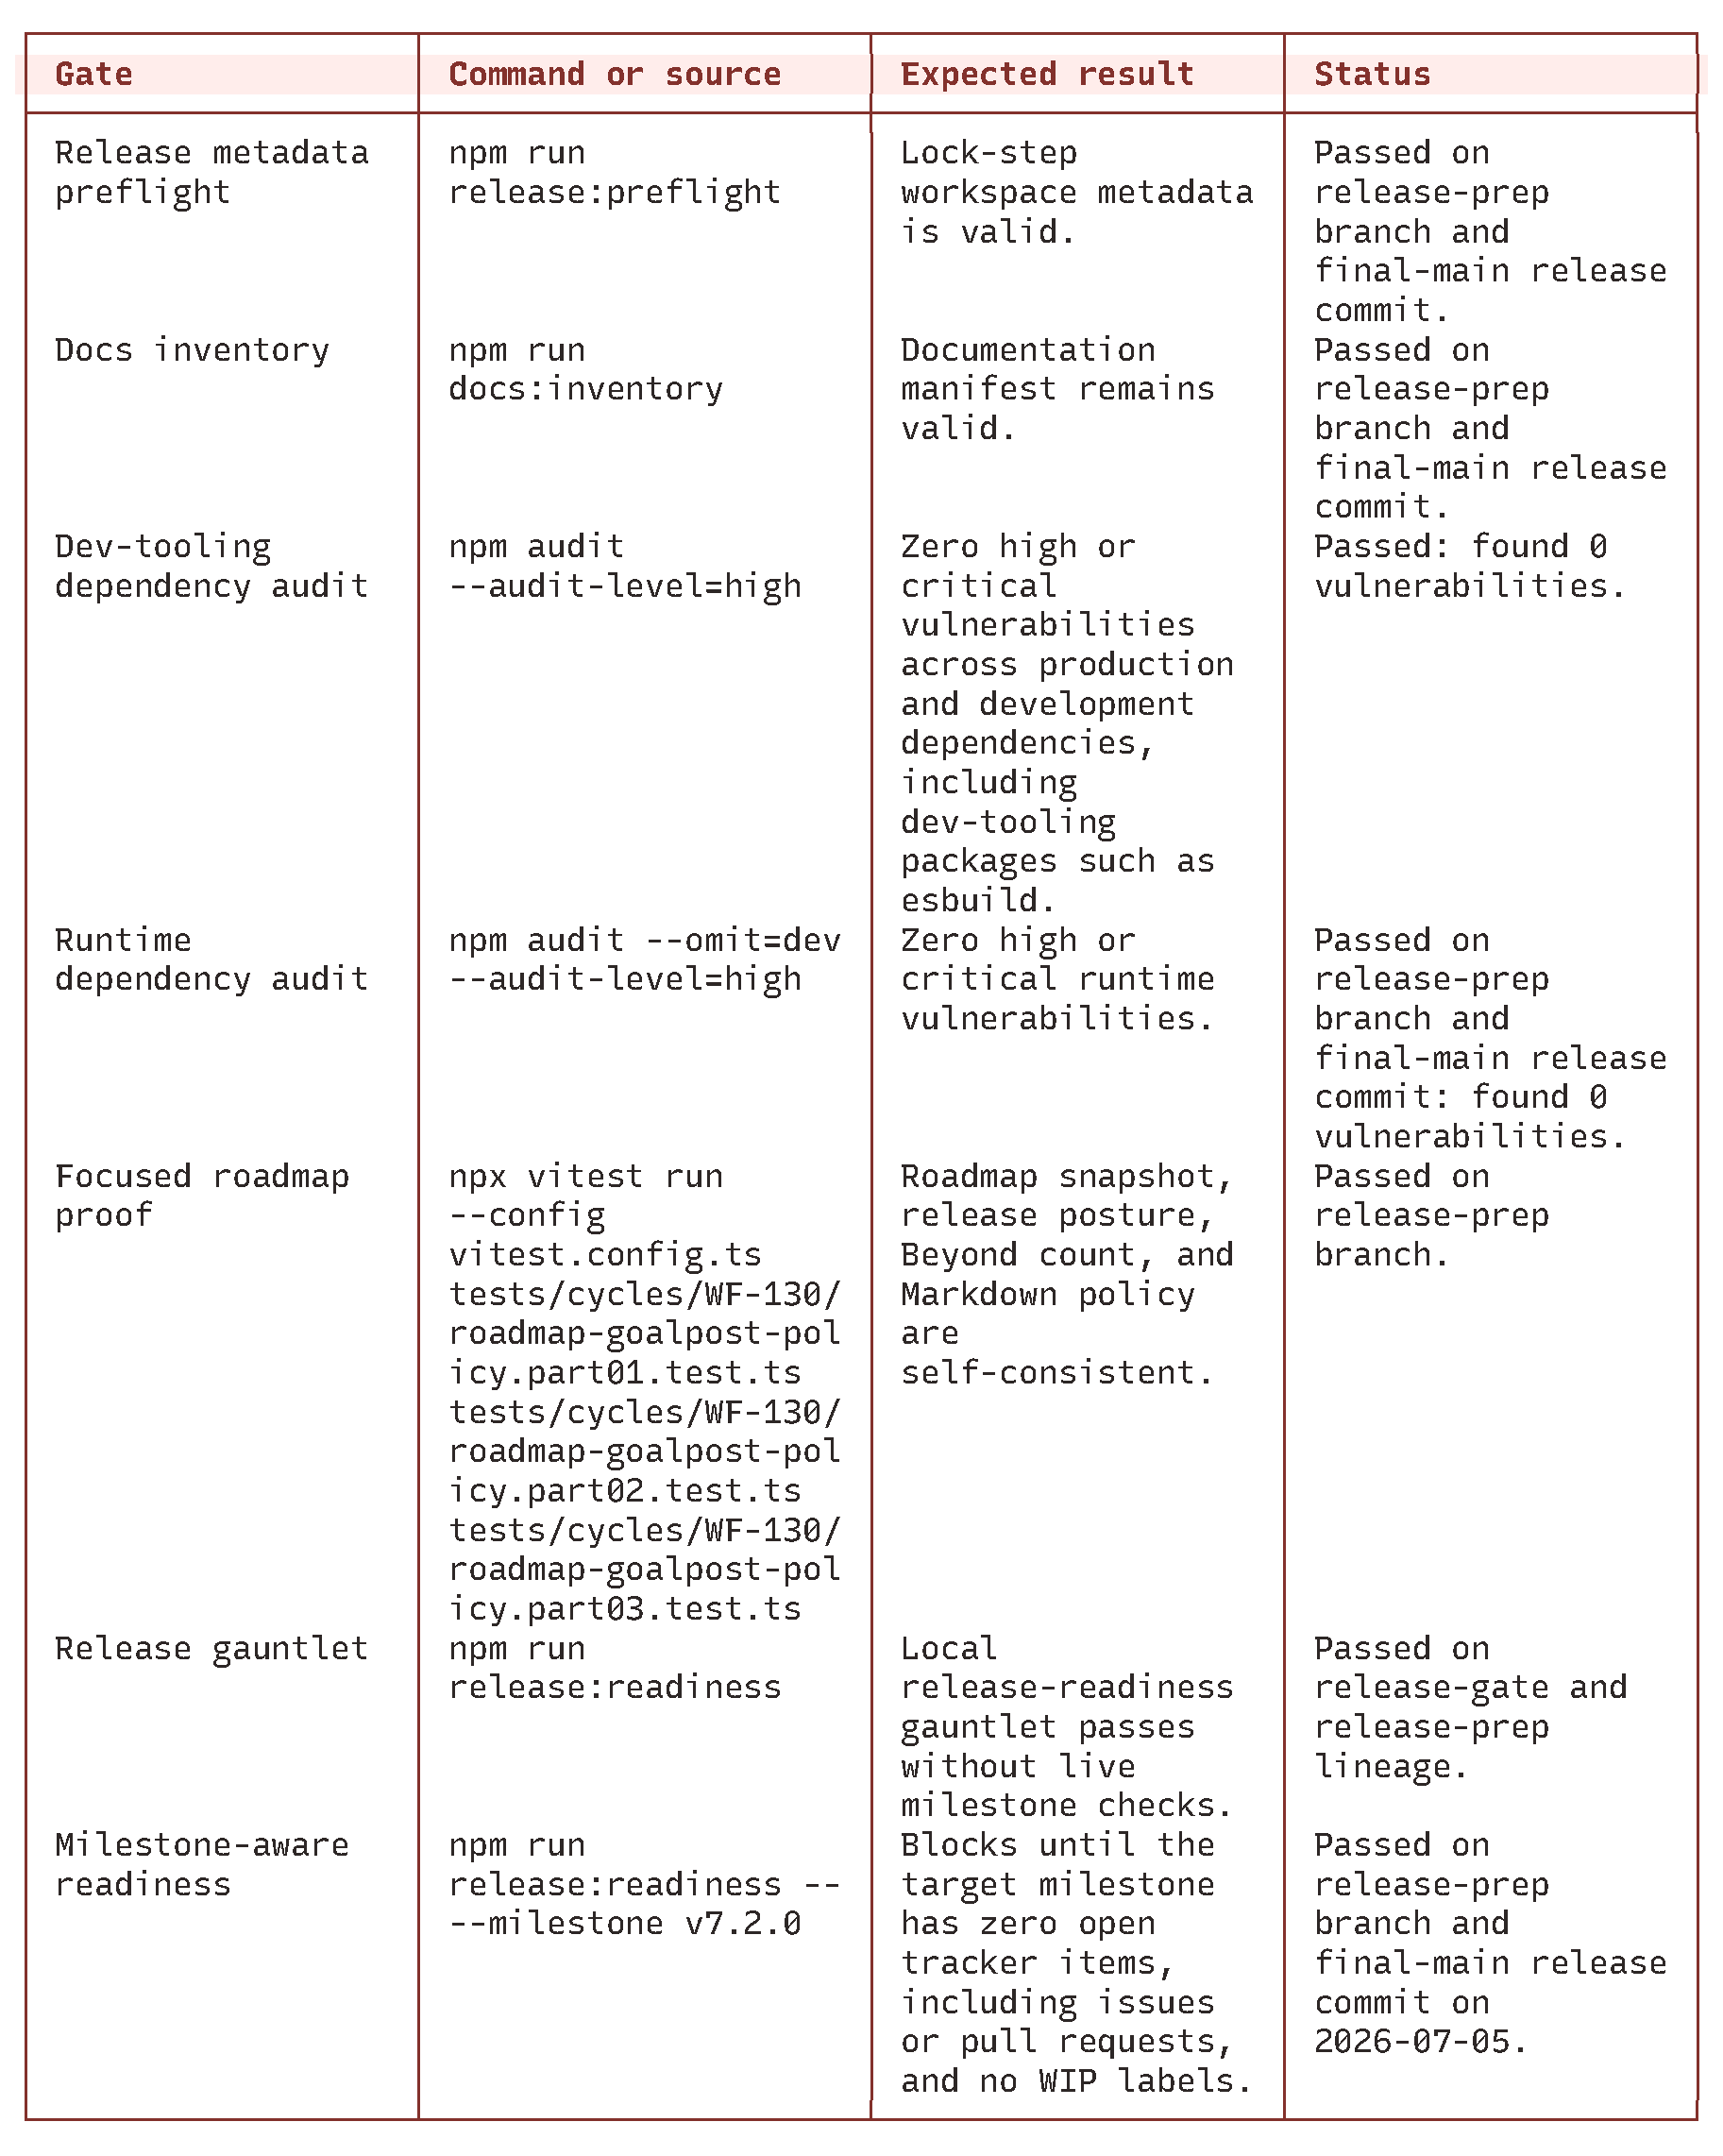
\includegraphics[width=\linewidth]{figures/tables/table-068-g1-1.pdf}
\par\smallskip{\scriptsize\color{BookMuted}Rows 1–7. Actual Bijou table component.}
\end{center}
\par\medskip
\begin{center}
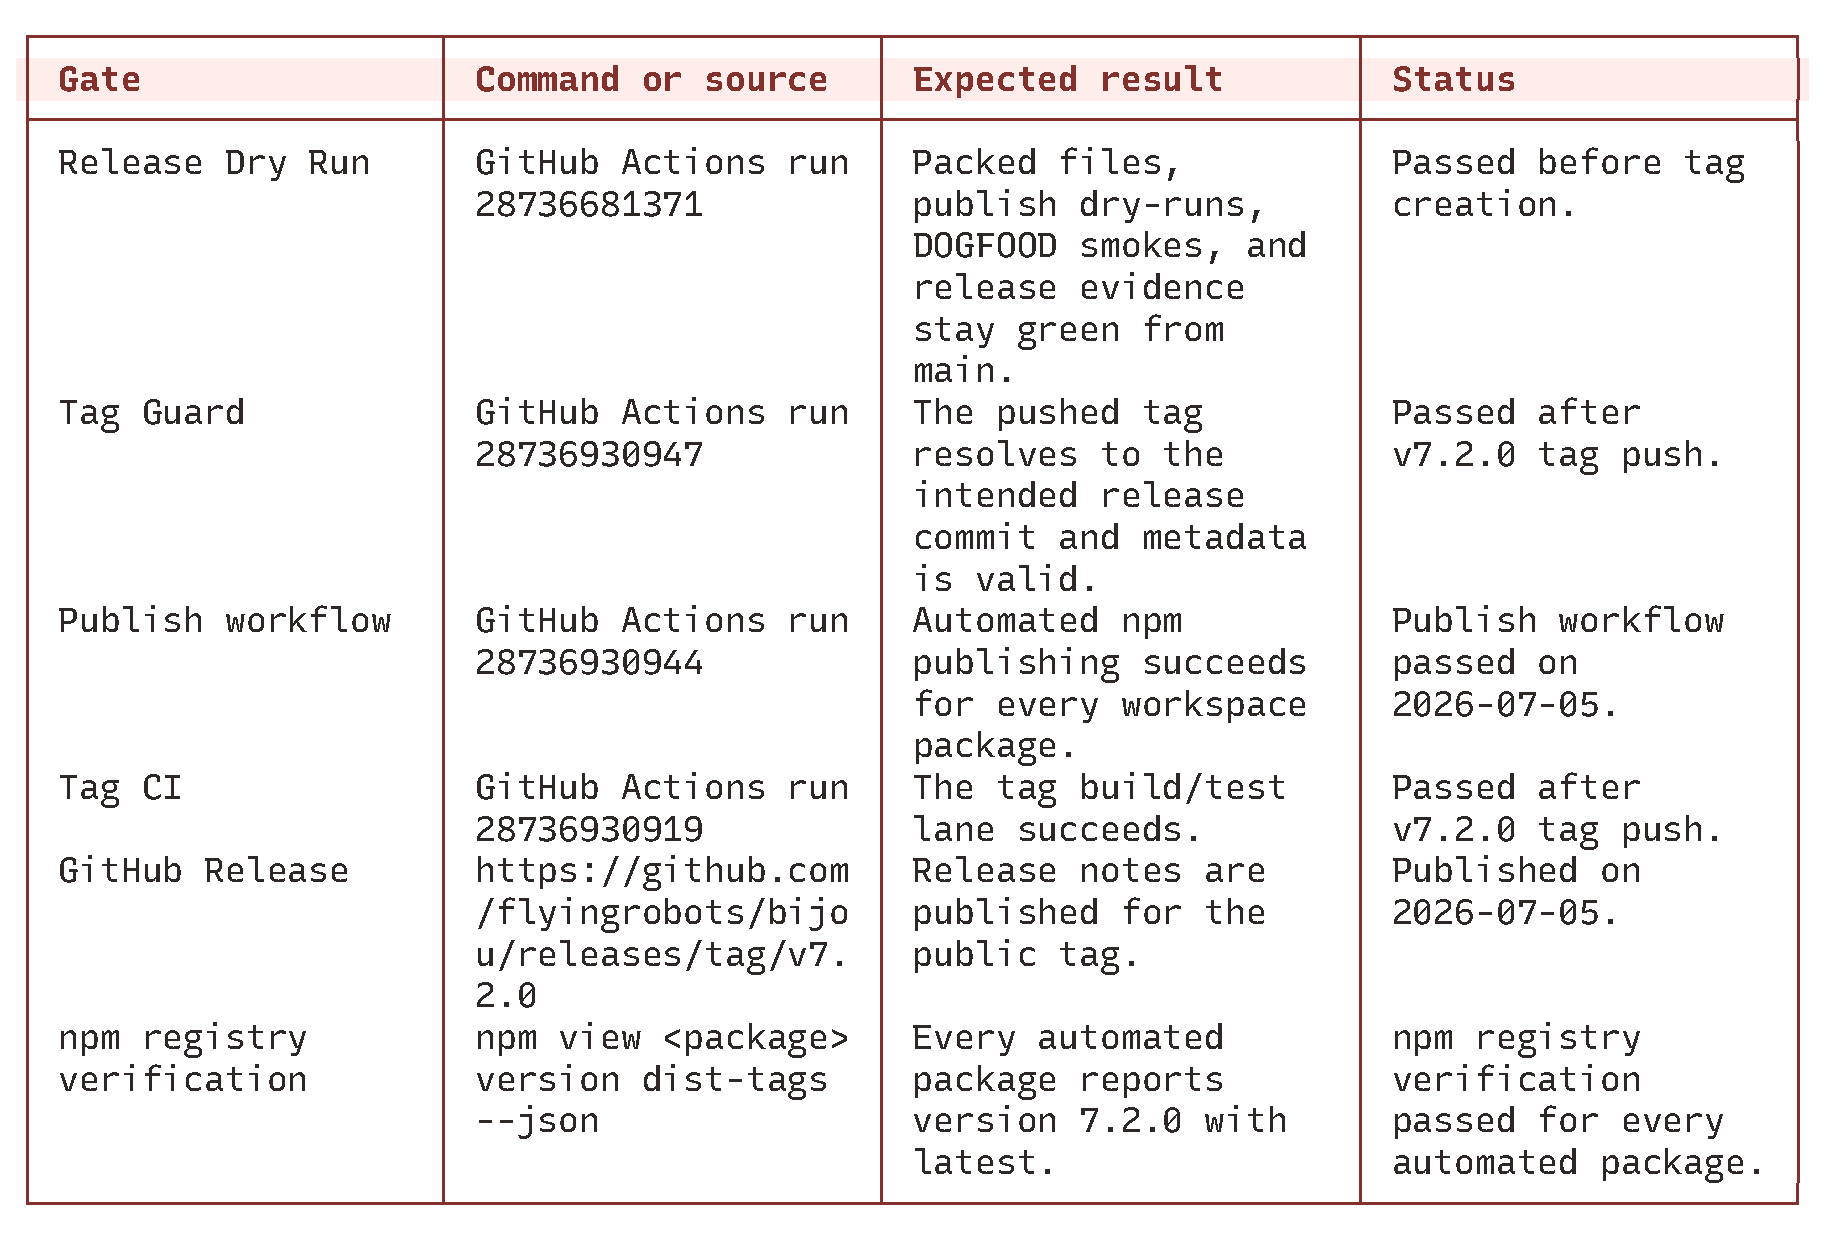
\includegraphics[width=\linewidth]{figures/tables/table-068-g1-2.pdf}
\par\smallskip{\scriptsize\color{BookMuted}Rows 8–13. Actual Bijou table component.}
\end{center}


\section{Human Review Matrix}\label{record-261-human-review-matrix}

\begin{center}
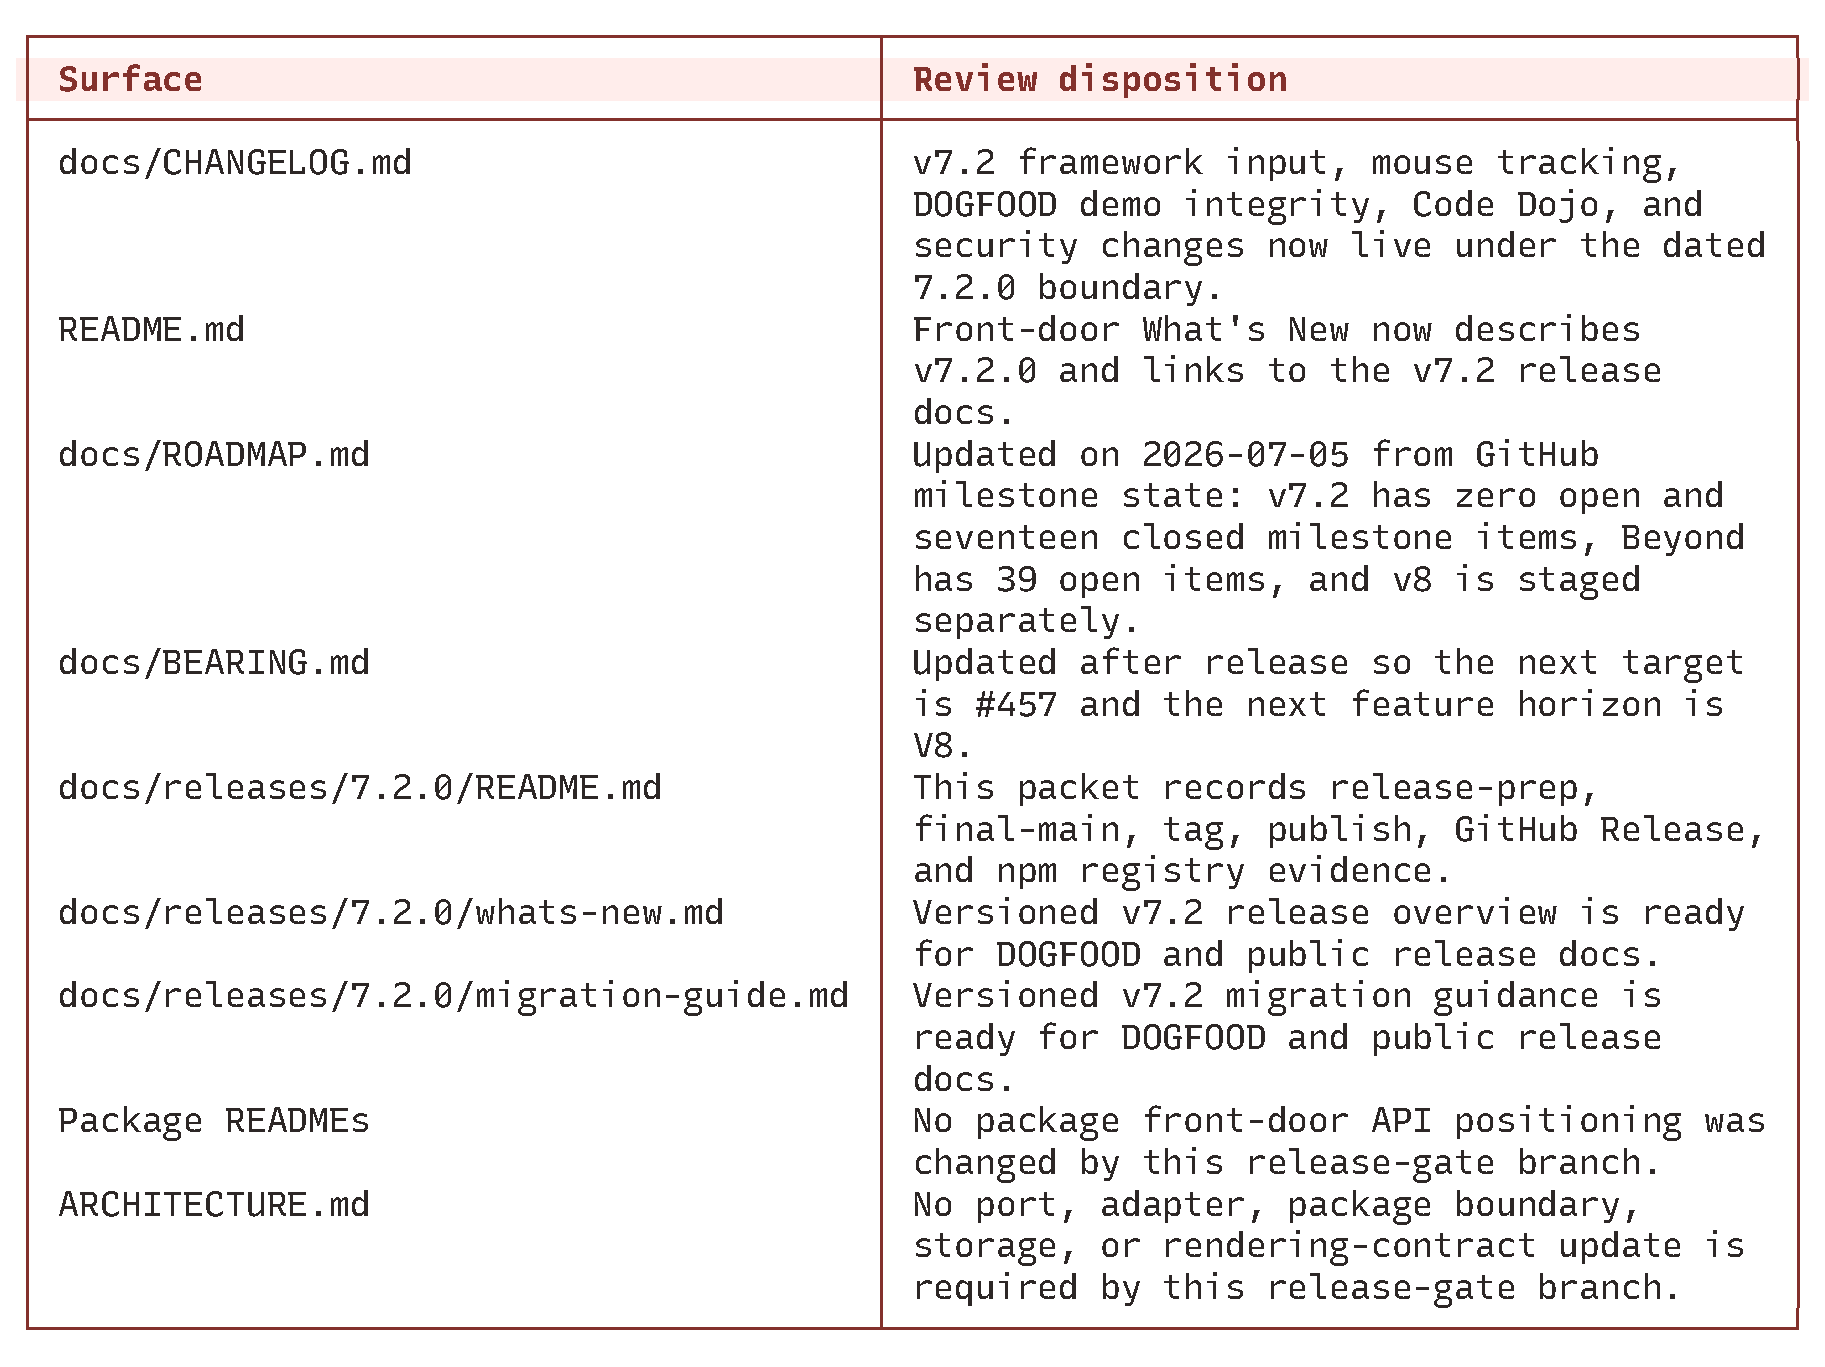
\includegraphics[width=\linewidth]{figures/tables/table-069-g1-1.pdf}
\par\smallskip{\scriptsize\color{BookMuted}Rows 1–9. Actual Bijou table component.}
\end{center}


\section{Package And Registry Verification Plan}\label{record-261-package-and-registry-verification-plan}

The release-prep PR performed the package metadata mutation and validated the resulting branch before it merged:

\begin{CodeBlock}
npm run version 7.2.0
npm install --package-lock-only --ignore-scripts
npm run release:preflight
npm run docs:inventory
npm audit --audit-level=high
npm run release:readiness -- --milestone v7.2.0
\end{CodeBlock}

The \textbf{Release Dry Run} workflow ran against release-prep before merge and again from final \texttt{m\allowbreak{}a\allowbreak{}i\allowbreak{}n} before tag creation. The final-main run \url{https://github.com/flyingrobots/bijou/actions/runs/28736681371} is the authoritative packed-file and npm publish dry-run evidence for the automated publish matrix.

After the release-prep PR merged and local \texttt{m\allowbreak{}a\allowbreak{}i\allowbreak{}n} exactly matched \texttt{o\allowbreak{}r\allowbreak{}i\allowbreak{}g\allowbreak{}i\allowbreak{}n\allowbreak{}/\allowbreak{}m\allowbreak{}a\allowbreak{}i\allowbreak{}n}, final tag preparation replayed the metadata and docs checks from the merged commit:

\begin{CodeBlock}
git fetch origin main --tags --prune
git switch main
git merge --ff-only origin/main
git status --porcelain=v1
git rev-parse HEAD origin/main
test "$(git rev-parse HEAD)" = "$(git rev-parse origin/main)"
npm run release:preflight
npm run docs:inventory
\end{CodeBlock}

After the \texttt{v\allowbreak{}7\allowbreak{}.\allowbreak{}2\allowbreak{}.\allowbreak{}0} tag was pushed and the publish workflow passed, registry verification confirmed every published package resolves to version \texttt{7\allowbreak{}.\allowbreak{}2\allowbreak{}.\allowbreak{}0} with the stable \texttt{l\allowbreak{}a\allowbreak{}t\allowbreak{}e\allowbreak{}s\allowbreak{}t} dist-tag:

\begin{CodeBlock}
npm view @flyingrobots/bijou version dist-tags --json
npm view @flyingrobots/bijou-node version dist-tags --json
npm view @flyingrobots/bijou-tui version dist-tags --json
npm view @flyingrobots/bijou-tui-app version dist-tags --json
npm view create-bijou-tui-app version dist-tags --json
npm view @flyingrobots/bijou-i18n version dist-tags --json
npm view @flyingrobots/bijou-i18n-tools version dist-tags --json
npm view @flyingrobots/bijou-i18n-tools-node version dist-tags --json
npm view @flyingrobots/bijou-i18n-tools-xlsx version dist-tags --json
npm view @flyingrobots/bijou-mcp version dist-tags --json
\end{CodeBlock}

\section{Release-Time Registry Snapshot}\label{record-261-release-time-registry-snapshot}

The table below is the immutable release evidence. It records the registry state observed during post-publish verification on 2026-07-05 after Release workflow run \texttt{2\allowbreak{}8\allowbreak{}7\allowbreak{}3\allowbreak{}6\allowbreak{}9\allowbreak{}3\allowbreak{}0\allowbreak{}9\allowbreak{}4\allowbreak{}4} completed at \texttt{2\allowbreak{}0\allowbreak{}2\allowbreak{}6\allowbreak{}-\allowbreak{}0\allowbreak{}7\allowbreak{}-\allowbreak{}0\allowbreak{}5\allowbreak{}T\allowbreak{}1\allowbreak{}0\allowbreak{}:\allowbreak{}0\allowbreak{}3\allowbreak{}:\allowbreak{}0\allowbreak{}4\allowbreak{}Z} from release commit \texttt{1\allowbreak{}2\allowbreak{}3\allowbreak{}f\allowbreak{}4\allowbreak{}a\allowbreak{}6\allowbreak{}1\allowbreak{}5\allowbreak{}0\allowbreak{}9\allowbreak{}6\allowbreak{}3\allowbreak{}9\allowbreak{}3\allowbreak{}2\allowbreak{}1\allowbreak{}1\allowbreak{}8\allowbreak{}c\allowbreak{}b\allowbreak{}f\allowbreak{}7\allowbreak{}6\allowbreak{}3\allowbreak{}a\allowbreak{}8\allowbreak{}a\allowbreak{}6\allowbreak{}e\allowbreak{}c\allowbreak{}0\allowbreak{}3\allowbreak{}4\allowbreak{}8\allowbreak{}7\allowbreak{}e\allowbreak{}2\allowbreak{}2\allowbreak{}7}. The \texttt{n\allowbreak{}p\allowbreak{}m\allowbreak{} \allowbreak{}v\allowbreak{}i\allowbreak{}e\allowbreak{}w} commands above are operational replay aids and may report a later \texttt{l\allowbreak{}a\allowbreak{}t\allowbreak{}e\allowbreak{}s\allowbreak{}t} value after a future release; this table is the historical \texttt{v\allowbreak{}7\allowbreak{}.\allowbreak{}2\allowbreak{}.\allowbreak{}0} snapshot.

\begin{center}
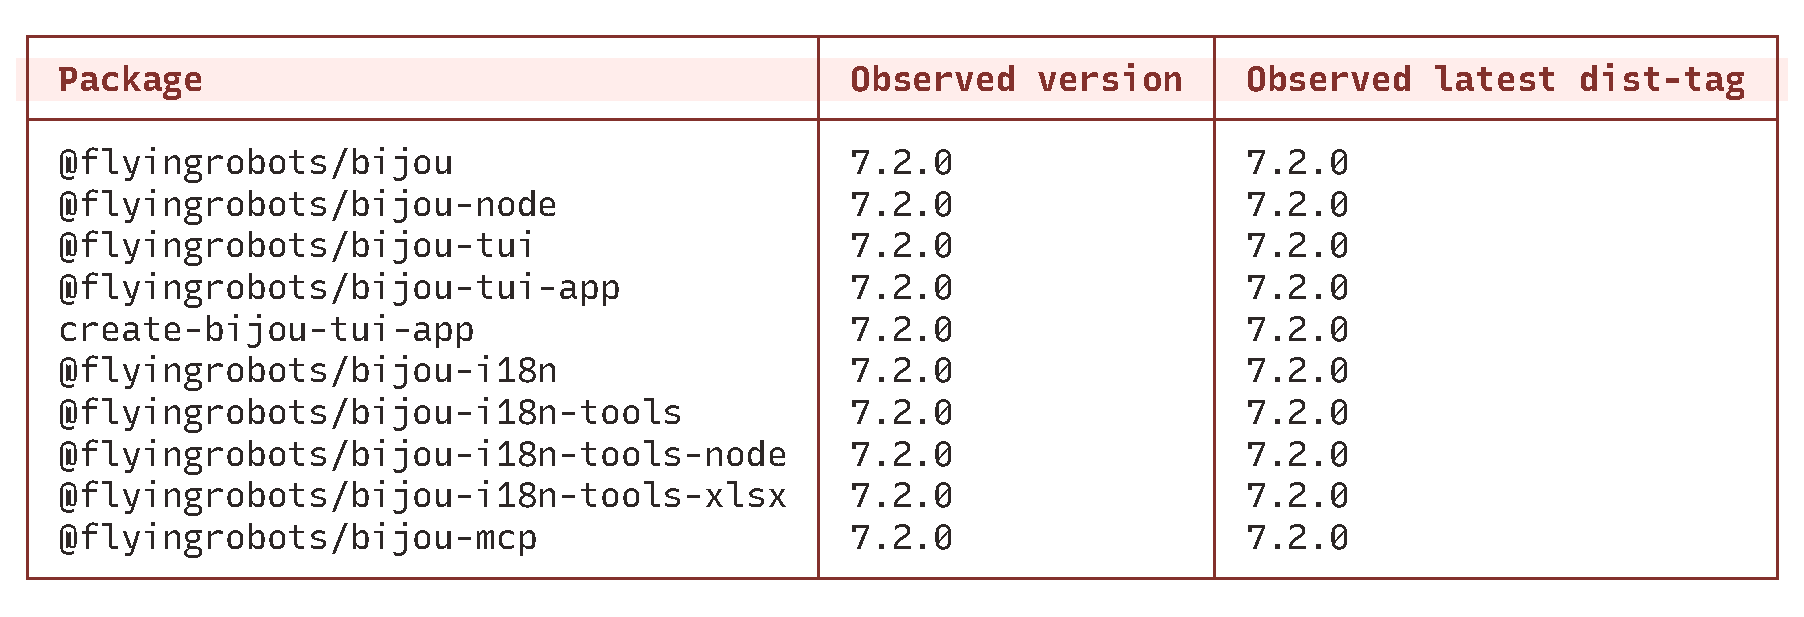
\includegraphics[width=\linewidth]{figures/tables/table-070-g1-1.pdf}
\par\smallskip{\scriptsize\color{BookMuted}Rows 1–10. Actual Bijou table component.}
\end{center}


Tag creation, publish automation, npm registry verification, and GitHub Release verification all ran from the merged release commit after the release-prep branch landed. The public release is \url{https://github.com/flyingrobots/bijou/releases/tag/v7.2.0}.

\section{Deterministic Reproducibility}\label{record-261-deterministic-reproducibility}

All historical release-prep claims above are replayable from the release-prep branch tip with:

\begin{CodeBlock}
npm run release:preflight
npm run docs:inventory
npm audit --audit-level=high
npm audit --omit=dev --audit-level=high
npx vitest run --config vitest.config.ts tests/cycles/WF-130/roadmap-goalpost-policy.part01.test.ts tests/cycles/WF-130/roadmap-goalpost-policy.part02.test.ts tests/cycles/WF-130/roadmap-goalpost-policy.part03.test.ts
npm run release:readiness
\end{CodeBlock}

The public tag was created only after the final merged \texttt{m\allowbreak{}a\allowbreak{}i\allowbreak{}n} checks passed:

\begin{CodeBlock}
npm run release:preflight
npm run docs:inventory
npm run release:readiness -- --milestone v7.2.0
npm audit --audit-level=high
npm audit --omit=dev --audit-level=high
\end{CodeBlock}

The final tag was created after \#354 closed, the release-prep PR merged, the local checkout was clean, \texttt{m\allowbreak{}a\allowbreak{}i\allowbreak{}n} exactly matched \texttt{o\allowbreak{}r\allowbreak{}i\allowbreak{}g\allowbreak{}i\allowbreak{}n\allowbreak{}/\allowbreak{}m\allowbreak{}a\allowbreak{}i\allowbreak{}n}, and CI / Release Dry Run evidence was green.

\section{Residual Risk}\label{record-261-residual-risk}

\begin{itemize}
\tightlist
\item
  Code Dojo debt remains tracked by ratcheting baselines. This release improves enforcement and lowers debt, but does not claim zero standards debt.
\end{itemize}

